% Author: Daniel Vartanian.
% Licence: MIT. See <https://opensource.org/license/mit/> to learn more.
%
% Based on: template.tex, developed by the Quarto team and
%   abtex2-modelo-trabalho-academico.tex, v-1.9.7, developed by
%   Lauro César Araujo and the team behind abnt2tex, with additional guidance
%   from the theses and dissertations regulations of the University of São Paulo
%   (USP). For more information, please visit <http://www.abntex.net.br/>.

% For help, see:
%
% - <https://quarto.org/docs/reference/formats/pdf.html>
% - <https://github.com/abntex/abntex2/wiki/ComoCustomizar>
% - <https://www.ctan.org/pkg/abntex2>
% - <https://www.ctan.org/pkg/memoir>
% - <https://www.ctan.org/pkg/hyperref>

% TO DO:
%
% * Slightly move the toc to the left, in a way that the spacing between titles
%   and numbers become the same as the textual chapters.
% * Remove hiperlink spans by page breaks. See: <https://tex.stackexchange.com/questions/54136/hyperref-link-spans-a-pagebreak-looks-ugly>.

% -----
% Preamble
% -----

% Don´t move the `\PassOptionsToPackage` macros.
% See why: <https://tex.stackexchange.com/a/433605/234832>.
\PassOptionsToPackage{
unicode,bookmarksnumbered
}{hyperref}

\PassOptionsToPackage{hyphens}{url}

\PassOptionsToPackage{dvipsnames,svgnames,x11names}{xcolor}


\documentclass[
12pt,
openright,
oneside,
a4paper,
chapter=TITLE,
section=TITLE,
french,
spanish,
brazil,
english
]{abntex2}
% \usepackage{showframe}

% The order in which the packages are loaded is important!

\usepackage{array}
\usepackage{calc}
\usepackage{caption}
\usepackage{color}
\usepackage{colortbl}
\usepackage{amsmath}
\usepackage{amssymb}
\usepackage{booktabs}
\usepackage{enumitem}
\usepackage{etoolbox}
\usepackage{epigraph}
\usepackage{float}
\usepackage[T1]{fontenc}
\usepackage[hang,multiple]{footmisc}
\usepackage{graphicx}
\usepackage{iftex}
\usepackage{indentfirst}
\usepackage[hyphenation,lastparline,nosingleletter]{impnattypo}
\usepackage[utf8]{inputenc}
\usepackage{lastpage}
\usepackage{lipsum}
\usepackage{longtable}
\usepackage{luacode}
\usepackage{luatexbase}
\usepackage{microtype}
\usepackage{multirow}
\usepackage{parskip}
\usepackage{pdfpages}
\usepackage{titlesec}
\usepackage[table]{xcolor}
\usepackage{xparse}
\usepackage{xstring}
\usepackage{hyperref}
\usepackage{url}

\ifPDFTeX
  \usepackage{textcomp} % provide euro and other symbols
\else % if luatex or xetex
\usepackage{unicode-math}
\fi
% Set lengths -----

\newlength{\microskipamount}
\newlength{\tinyskipamount}
\newlength{\hugeskipamount}

\setlength{\microskipamount}{0.25\baselineskip} % Arial/12pt/1.5 == 5.4375pt
\setlength{\tinyskipamount}{0.5\baselineskip} % Arial/12pt/1.5 == 10.875pt
\setlength{\smallskipamount}{0.75\baselineskip} % Arial/12pt/1.5 == 16.3125pt
\setlength{\medskipamount}{1\baselineskip} % Arial/12pt/1.5 == 21.75pt
\setlength{\bigskipamount}{1.5\baselineskip} % Arial/12pt/1.5 == 32.625pt
\setlength{\hugeskipamount}{2\baselineskip}% Arial/12pt/1.5 == 43.5pt

\newcommand{\microskip}{\vspace{\microskipamount}}
\newcommand{\tinyskip}{\vspace{\tinyskipamount}}
\newcommand{\hugeskip}{\vspace{\hugeskipamount}}

% Set skips -----

\setlength{\beforechapskip}{\bigskipamount}
\setlength{\afterchapskip}{\smallskipamount}

\titlespacing*{\chapter}{0pt}{\beforechapskip}{\afterchapskip}
\titlespacing*{\section}{0pt}{\medskipamount}{\smallskipamount}
\titlespacing*{\subsection}{0pt}{\medskipamount}{\smallskipamount}
\titlespacing*{\subsubsection}{0pt}{\medskipamount}{\smallskipamount}
\titlespacing*{\paragraph}{0pt}{\medskipamount}{\smallskipamount}

% Set epigraph -----

\setlength\epigraphwidth{0.6\textwidth}
\setlength\epigraphrule{0pt}
% Set page -----

\setlength{\headsep}{1cm}
\setlength{\footskip}{1cm}
\checkandfixthelayout[fixed]

% Set text spacing -----

\renewcommand{\familydefault}{\rmdefault}

\renewcommand{\baselinestretch}{1.5}

\setlength{\parindent}{1cm}

\setlength{\parskip}{0ex}

% Set text font -----


\ifPDFTeX\else
    % xetex/luatex font selection
  \setmainfont[]{Poppins}
  \setsansfont[]{Poppins}
  \setmonofont[Scale=0.75]{DM Mono}




\fi


% Set footnote -----

\setlength{\footnotemargin}{0.5em} % Equal to `\footmarkwidth`
\let\svfootnoterule\footnoterule % Equal to `\footmarksep`
\renewcommand\footnoterule{\vspace{1ex}\svfootnoterule\vspace{1ex}}
\newcommand{\capaname}{Capa}
\newcommand{\fichacatalograficaname}{Ficha catalográfica}
\newcommand{\resumoestrangeironame}{Resumo}
\newcommand{\glossarioname}{Glossário}

\addto\captionsenglish{
  \renewcommand{\capaname}{Cover}
  \renewcommand{\folhaderostoname}{Title Page}
  \renewcommand{\fichacatalograficaname}{Cataloging Record}
  \renewcommand{\errataname}{Errata}
  \renewcommand{\folhadeaprovacaoname}{Approval Sheet}
  \renewcommand{\dedicatorianame}{Inscription}
  \renewcommand{\agradecimentosname}{Acknowledgements}
  \renewcommand{\epigraphname}{Epigraph}
  \renewcommand{\resumoname}{Abstract}
  \renewcommand{\resumoestrangeironame}{Resumo}
  \renewcommand{\listfigurename}{List of Figures}
  \renewcommand{\listtablename}{List of Tables}
  \renewcommand{\listadesiglasname}{List of Abbreviations and Acronyms}
  \renewcommand{\listadesimbolosname}{List of Symbols}
  \renewcommand{\contentsname}{Contents}
  \renewcommand{\bibname}{References}
  \renewcommand{\glossarioname}{Glossary}
  \renewcommand{\apendicename}{APPENDIX}
  \renewcommand{\apendicesname}{Appendices}
  \renewcommand{\anexoname}{ANNEX}
  \renewcommand{\anexosname}{Annexes}
  \renewcommand{\indexname}{Index}
  \renewcommand{\orientadorname}{Supervisor:}
  \renewcommand{\coorientadorname}{Co-supervisor:}
  \renewcommand{\fontename}{Source}
  \renewcommand{\notaname}{Note}
  \renewcommand{\pageautorefname}{page}
  \renewcommand{\sectionautorefname}{section}
  \renewcommand{\subsectionautorefname}{subsection}
  \renewcommand{\subsubsectionautorefname}{subsubsection}
  \renewcommand{\paragraphautorefname}{subsubsubsection}
}

\addto\captionsbrazil{
  \renewcommand{\capaname}{Capa}
  \renewcommand{\folhaderostoname}{Folha de Rosto}
  \renewcommand{\fichacatalograficaname}{Ficha Catalográfica}
  \renewcommand{\errataname}{Errata}
  \renewcommand{\folhadeaprovacaoname}{Folha de Aprovação}
  \renewcommand{\dedicatorianame}{Dedicatória}
  \renewcommand{\agradecimentosname}{Agradecimentos}
  \renewcommand{\epigraphname}{Epígrafe}
  \renewcommand{\resumoname}{Resumo}
  \renewcommand{\resumoestrangeironame}{Abstract}
  \renewcommand{\listfigurename}{Lista de Figuras}
  \renewcommand{\listtablename}{Lista de Tabelas}
  \renewcommand{\listadesiglasname}{Lista de Abreviaturas e Siglas}
  \renewcommand{\listadesimbolosname}{Lista de Símbolos}
  \renewcommand{\contentsname}{Sumário}
  \renewcommand{\bibname}{Referências}
  \renewcommand{\glossarioname}{Glossário}
  \renewcommand{\apendicename}{APÊNDICE}
  \renewcommand{\apendicesname}{Apêndices}
  \renewcommand{\anexoname}{ANEXO}
  \renewcommand{\anexosname}{Anexos}
  \renewcommand{\indexname}{Índice}
  \renewcommand{\orientadorname}{Orientador:}
  \renewcommand{\coorientadorname}{Coorientador:}
  \renewcommand{\fontename}{Fonte}
  \renewcommand{\notaname}{Nota}
  \renewcommand{\pageautorefname}{página}
  \renewcommand{\sectionautorefname}{seção}
  \renewcommand{\subsectionautorefname}{subseção}
  \renewcommand{\subsubsectionautorefname}{subsubseção}
  \renewcommand{\paragraphautorefname}{subsubsubseção}
}

\addto\captionsspanish{
  \renewcommand{\capaname}{Portada}
  \renewcommand{\folhaderostoname}{Página de título}
  \renewcommand{\fichacatalograficaname}{Ficha Catalográfica}
  \renewcommand{\errataname}{Errata}
  \renewcommand{\folhadeaprovacaoname}{Hoja de aprobación}
  \renewcommand{\dedicatorianame}{Dedicatoria}
  \renewcommand{\agradecimentosname}{Agradecimientos}
  \renewcommand{\epigraphname}{Epígrafe}
  \renewcommand{\resumoname}{Resumen}
  \renewcommand{\resumoestrangeironame}{Resumo}
  \renewcommand{\listfigurename}{Lista de Figuras}
  \renewcommand{\listtablename}{Lista de Tablas}
  \renewcommand{\listadesiglasname}{Lista de Abreviaturas y Siglas}
  \renewcommand{\listadesimbolosname}{Lista de Símbolos}
  \renewcommand{\contentsname}{Sumario}
  \renewcommand{\bibname}{Referencias}
  \renewcommand{\glossarioname}{Glosario}
  \renewcommand{\apendicename}{APÉNDICE}
  \renewcommand{\apendicesname}{Apéndices}
  \renewcommand{\anexoname}{ANEXO}
  \renewcommand{\anexosname}{Anexos}
  \renewcommand{\indexname}{Índice}
  \renewcommand{\orientadorname}{Asesor:}
  \renewcommand{\coorientadorname}{Coasesor:}
  \renewcommand{\fontename}{Fuente}
  \renewcommand{\notaname}{Nota}
  \renewcommand{\pageautorefname}{página}
  \renewcommand{\sectionautorefname}{sección}
  \renewcommand{\subsectionautorefname}{subsección}
  \renewcommand{\subsubsectionautorefname}{subsubsección}
  \renewcommand{\paragraphautorefname}{subsubsubsección}
}

\addto\captionsfrench{
  \renewcommand{\capaname}{Couverture}
  \renewcommand{\folhaderostoname}{Page de Titre}
  \renewcommand{\fichacatalograficaname}{Fiche Cataloguée}
  \renewcommand{\errataname}{Errata}
  \renewcommand{\folhadeaprovacaoname}{Feuille d'Approbation}
  \renewcommand{\dedicatorianame}{Dédiace
  \renewcommand{\agradecimentosname}{Remerciements}}
  \renewcommand{\epigraphname}{Épigraphe}
  \renewcommand{\resumoname}{Résumé}
  \renewcommand{\resumoestrangeironame}{Resumo}
  \renewcommand{\listfigurename}{Liste des Figures}
  \renewcommand{\listtablename}{Liste des Tableaux}
  \renewcommand{\listadesiglasname}{Liste des Abréviations et Sigles}
  \renewcommand{\listadesimbolosname}{Liste des Symboles}
  \renewcommand{\contentsname}{Sommaire}
  \renewcommand{\bibname}{Références}
  \renewcommand{\glossarioname}{Glossaire}
  \renewcommand{\apendicename}{APPENDICE}
  \renewcommand{\apendicesname}{Appendices}
  \renewcommand{\anexoname}{ANNEXE}
  \renewcommand{\anexosname}{Annexes}
  \renewcommand{\indexname}{Index}
  \renewcommand{\orientadorname}{Conseiller:}
  \renewcommand{\coorientadorname}{Co-conseiller:}
  \renewcommand{\fontename}{Source}
  \renewcommand{\notaname}{Note}
  \renewcommand{\pageautorefname}{page}
  \renewcommand{\sectionautorefname}{section}
  \renewcommand{\subsectionautorefname}{sous-section}
  \renewcommand{\subsubsectionautorefname}{sous-sous-section}
  \renewcommand{\paragraphautorefname}{sous-sous-sous-section}
}
% See `babel.tex` for language changes.
% See `toc.text` for changes related to the ToC.

% Set page numbering -----

\makepagestyle{abntheadings}
\makeevenhead{abntheadings}{\ABNTEXfontereduzida\thepage}{}{}
\makeoddhead{abntheadings}{}{}{\ABNTEXfontereduzida\thepage}

% Set text variables -----

\renewcommand{\ABNTEXpartfont}{\sffamily\bfseries}
\renewcommand{\ABNTEXpartfontsize}{\normalsize}
\renewcommand{\ABNTEXchapterfont}{\sffamily\bfseries}
\renewcommand{\ABNTEXchapterfontsize}{\normalsize}
\renewcommand{\ABNTEXsectionfont}{\sffamily}
\renewcommand{\ABNTEXsectionfontsize}{\normalsize}
\renewcommand{\ABNTEXsubsectionfont}{\sffamily}
\renewcommand{\ABNTEXsubsectionfontsize}{\normalsize}
\renewcommand{\ABNTEXsubsubsectionfont}{\sffamily}
\renewcommand{\ABNTEXsubsubsectionfontsize}{\normalsize}
\renewcommand{\ABNTEXsubsubsubsectionfont}{\sffamily}
\renewcommand{\ABNTEXsubsubsubsectionfontsize}{\normalsize\itshape}
\renewcommand{\ABNTEXfontereduzida}{\footnotesize}
\renewcommand{\ABNTEXcaptiondelim}{~\textendash~}
\renewcommand{\ABNTEXcaptionfontedelim}{:~}

\renewcommand{\captiontitlefont}{\ABNTEXfontereduzida}

% Set new commands -----

\providecommand{\imprimiruniversidade}{}
\newcommand{\universidade}[1]{\renewcommand{\imprimiruniversidade}{#1}}

\providecommand{\imprimirescola}{}
\newcommand{\escola}[1]{\renewcommand{\imprimirescola}{#1}}

\providecommand{\imprimirprograma}{}
\newcommand{\programa}[1]{\renewcommand{\imprimirprograma}{#1}}

\newcommand{\imprimirtipodetrabalho}{\imprimirtipotrabalho}

\providecommand{\imprimirtipodetituloacademico}{}
\newcommand{\tipodetituloacademico}[1]{\renewcommand{\imprimirtipodetituloacademico}{#1}}

\providecommand{\imprimirtituloacademico}{}
\newcommand{\tituloacademico}[1]{\renewcommand{\imprimirtituloacademico}{#1}}

\providecommand{\imprimirareadeconcentracao}{}
\newcommand{\areadeconcentracao}[1]{\renewcommand{\imprimirareadeconcentracao}{#1}}

\providecommand{\imprimirnotadeversao}{}
\newcommand{\notadeversao}[1]{\renewcommand{\imprimirnotadeversao}{#1}}

% Set chapter style -----

\renewcommand{\chapnamefont}{\ABNTEXchapterfont\ABNTEXchapterfontsize\mdseries}
\renewcommand{\chapnumfont}{\ABNTEXchapterfont\ABNTEXchapterfontsize\mdseries}

\setsecnumformat{\chapnumfont\csname the#1\endcsname\quad}

\renewcommand{\printchaptername}{
  \ifthenelse{\boolean{abntex@apendiceousecao}}{
    \vspace*{\medskipamount}
    \chapnamefont \ABNTEXchapterupperifneeded{\appendixname} % [Changed]
  }{}
}

% Open an issue about it (`\hspace{-1em}`) - Title streching.
\renewcommand{\chapternamenum}{
  \ifthenelse{\boolean{abntex@apendiceousecao}}{
    \hspace{-2em} \space
  }{}
}

\renewcommand{\printchapternum}{
  \tocprintchapter
  \setboolean{abntex@innonumchapter}{false}
  \chapnumfont
  \thechapter % [Changed]
  % \ifthenelse{\boolean{abntex@apendiceousecao}}{ % [Removed]
  %   \tocinnonumchapter
  %   \ABNTEXcaptiondelim
  % }{}
}

\renewcommand{\afterchapternum}{
  \ifthenelse{\boolean{abntex@apendiceousecao}}{ % [Added]
    \ABNTEXchapterfont\mdseries \hspace{-1em} \space\ABNTEXcaptiondelim\space \hspace{-1.5em}
  }{
    \hspace{-0.875em}
  }
}

\renewcommand{\printchapternonum}{
  \tocprintchapternonum
  \setlength{\afterchapskip}{\hugeskipamount} % [Added]
  \setboolean{abntex@innonumchapter}{true}
}

\renewcommand{\printchaptertitle}[1]{
  \chaptitlefont
  \ifthenelse{\boolean{abntex@innonumchapter}}{
    \centering \ABNTEXchapterupperifneeded{#1}
  }{
    \ifthenelse{\boolean{abntex@apendiceousecao}}{
      \ABNTEXchapterfont\mdseries\ABNTEXchapterupperifneeded{#1}
    }{
      \ABNTEXchapterupperifneeded{#1}
    }
  }
}

% Set `\textual` -----

\renewcommand{\textual}{
  \pagestyle{abntheadings}
  \aliaspagestyle{chapter}{abntheadings}
}

% Set cover -----

\renewcommand{\imprimircapa}{
  \phantomsection\pdfbookmark[0]{\capaname}{}
  \begin{capa}%
  \begin{adjustwidth}{-1cm}{0cm}
  \center
  \imprimirinstituicao

  \vfill
  \imprimirautor

  \vfill
  {\ABNTEXchapterfont\imprimirtitulo}

  \vfill
  \vspace{6.5cm}
  \imprimirlocal

  \imprimirdata
  \vspace{1.5cm}
  \end{adjustwidth}
  \end{capa}
}

% Set title page -----

\makeatletter
\renewcommand{\folhaderostocontent}{
  \begin{center}
  \imprimirautor

  \vfill
  {\ABNTEXchapterfont\imprimirtitulo}

  \vfill
  \textbf{\imprimirnotadeversao}

  \vfill
  \abntex@ifnotempty{
    \imprimirpreambulo
  }{
    \hspace{0.35\textwidth}
    \begin{minipage}{.6\textwidth}
    \SingleSpacing
    \imprimirpreambulo
    \end{minipage}
  }

  \vfill
  \imprimirlocal

  \imprimirdata
  \vspace{1cm}
  \end{center}
}
\makeatother

% Set cataloging record -----

\renewenvironment{fichacatalografica}{
  \PRIVATEbookmarkthis{\fichacatalograficaname}
  \setlength{\parindent}{0cm}
  \begin{SingleSpacing}
}{
  \end{SingleSpacing}
}

% Set errata -----

\renewenvironment{errata}[1][\errataname]{
  \newpage
  \phantomsection
  \pretextualchapter{#1}
}{
  \cleardoublepage
}

% Set approval sheet -----

\renewenvironment{folhadeaprovacao}[1][\folhadeaprovacaoname]{
  \clearpage
  \PRIVATEbookmarkthis{#1}
  \setlength\parindent{0cm}
  \AtBeginEnvironment{tabular}{\normalsize}
  \begin{SingleSpace}
}{
  \end{SingleSpace}
  \cleardoublepage
}

% Set abstract -----

\newenvironment{resumoenv}[1][\resumoname]{
  \pretextualchapter{#1}
  \begingroup
  \setlength{\parindent}{0cm}
  \setlength{\parskip}{\smallskipamount} % The troublemaker.
  \AtBeginEnvironment{tabular}{\normalsize}
  \renewcommand{\arraystretch}{1}
  \setlength{\aboverulesep}{0ex}
  \setlength{\belowrulesep}{0ex}
  \setlength{\arrayrulewidth}{0pt}
  \setlength{\tabcolsep}{0cm}
  \vspace{-\smallskipamount} % !
  \begin{SingleSpace}
}{
  \end{SingleSpace}
  \cleardoublepage
  \endgroup
}

% Set list of abbreviations and acronyms -----

\renewenvironment{siglas}{
  \pretextualchapter{\listadesiglasname}
}{
  \cleardoublepage
}

% Set list of symbols -----

\renewenvironment{simbolos}{
  \pretextualchapter{\listadesimbolosname}
}{
  \cleardoublepage
}

% Set glossary -----

\newenvironment{glossario}{
  \tocprintchapternonum
}{
  \cleardoublepage
}

% Set appendices and annexes -----

\renewcommand{\PRIVATEapendiceconfig}[2]{
  \setboolean{abntex@apendiceousecao}{true}
  \renewcommand{\appendixname}{#1}
  %\renewcommand{\apendicesname}{#1}

  \ifthenelse{\boolean{ABNTEXsumario-abnt-6027-2012}}{
    \renewcommand{\appendixtocname}{\uppercase{#2}}
  }{
    \renewcommand{\appendixtocname}{#2}
  }

  \renewcommand{\appendixpagename}{#2}
  \renewcommand{\appendixtocname}{#2}
  % \switchchapname{#1} % [Altered]
  \renewcommand{\cftappendixname}{} % [Altered]
  \tocpartapendices % [Added]

  % Note:
  %
  % \cleardoublepage
  % \phantomsection
  % \addcontentsline{toc}{part}{Appendices}
  % \appendix
  %
  % is automatically add by the Quarto render.
}

\newcommand{\PRIVATEapendiceconfigafter}[1]{
    \chapterstyle{apendice}
    %\begingroup\centering\bfseries
    %\ABNTEXchapterupperifneeded{#1}
    %\par\endgroup
    %\vspace{\medskipamount}
    \pretextualchapter{#1}
    \let\clearpage\relax
}

\renewcommand{\apendices}{
  \clearpage
  \PRIVATEapendiceconfig{\apendicename}{\apendicesname}
  \appendix
  \PRIVATEapendiceconfigafter{\apendicesname}
}

\renewenvironment{apendicesenv}{
  \clearpage
  \PRIVATEapendiceconfig{\apendicename}{\apendicesname}
  \begin{appendix}
  \PRIVATEapendiceconfigafter{\apendicesname}
}{
  \end{appendix}
  \setboolean{abntex@apendiceousecao}{false}
  \bookmarksetup{startatroot}
}

\renewcommand{\anexos}{
  \clearpage
  % \cftinserthook{toc}{AAA} [Removed]
  \PRIVATEapendiceconfig{\anexoname}{\anexosname}

  \newpage % [Added]
  \phantomsection % [Added]
  \addcontentsline{toc}{part}{\appendixtocname} % [Added]

  \appendix
  \renewcommand\theHchapter{anexochapback.\arabic{chapter}}
  \PRIVATEapendiceconfigafter{\anexosname}
}

\renewenvironment{anexosenv}{
  \clearpage
  \PRIVATEapendiceconfig{\anexoname}{\anexosname}

  \newpage % [Added]
  \phantomsection % [Added]
  \addcontentsline{toc}{part}{\appendixtocname} % [Added]

  \begin{appendix}
  \renewcommand\theHchapter{anexochapback.\arabic{chapter}}
  \PRIVATEapendiceconfigafter{\anexosname}
}{
  \end{appendix}
  \setboolean{abntex@apendiceousecao}{false}
  \bookmarksetup{startatroot}
}
% -----
% New colors
% -----

\definecolor{blue}{HTML}{2905C3}

% See <https://getbootstrap.com/docs/5.0/utilities/colors/>.
\definecolor{quarto-blue}{HTML}{2780E3}
\definecolor{quarto-lighter-blue}{HTML}{ECF4FC}
\definecolor{quarto-orange}{HTML}{FF7518}
\definecolor{quarto-ligther-orange}{HTML}{FFF3EB}
\definecolor{quarto-red}{HTML}{D9534F}
\definecolor{quarto-ligther-red}{HTML}{FCF1F1}
\definecolor{quarto-green}{HTML}{3FB618}
\definecolor{quarto-ligther-green}{HTML}{EFF9EB}
\definecolor{quarto-purple}{HTML}{7D12BA}
\definecolor{quarto-gray}{HTML}{A3A3A3}
\definecolor{quarto-medium-gray}{HTML}{CFD0D1}
\definecolor{quarto-ligther-gray}{HTML}{F1F3F5}

\definecolor{bs-link-color}{HTML}{39729E}

% -----
% Body color
% -----

\definecolor{body-color}{HTML}{142A32}
\color{body-color}

% Quarto's default settings -----

% \usepackage{graphicx} % Already loaded in `packages.tex`.
\makeatletter
\newsavebox\pandoc@box
\newcommand*\pandocbounded[1]{% scales image to fit in text height/width
  \sbox\pandoc@box{#1}%
  \Gscale@div\@tempa{\textheight}{\dimexpr\ht\pandoc@box+\dp\pandoc@box\relax}%
  \Gscale@div\@tempb{\linewidth}{\wd\pandoc@box}%
  \ifdim\@tempb\p@<\@tempa\p@\let\@tempa\@tempb\fi% select the smaller of both
  \ifdim\@tempa\p@<\p@\scalebox{\@tempa}{\usebox\pandoc@box}%
  \else\usebox{\pandoc@box}%
  \fi%
}
% Set default figure placement to htbp
\def\fps@figure{htbp}
\makeatother

% Set distance from top of page to first float -----

\makeatletter
\setlength{\@fptop}{5pt}
\makeatother

% Set captions and legends -----

\DeclareCaptionFont{ABNTEXfontereduzida}{\ABNTEXfontereduzida}

% For customization, see `\DeclareCaptionFormat` in the `caption` package.
\captionsetup{
  font=ABNTEXfontereduzida
  ,justification=justified
}

\renewcommand{\abovecaptionskip}{\smallskipamount}
\renewcommand{\belowcaptionskip}{\smallskipamount}

\renewcommand{\legend}[1]{
  \hyphenpenalty=100000
  \ABNTEXfontereduzida
  \addvspace{\smallskipamount}
  #1
}

% Credits: <https://tex.stackexchange.com/a/611556/234832>.
\AddToHook{cmd/caption/before}{\hyphenpenalty=100000}

% Set figure environment -----

\AtBeginEnvironment{figure}{
  \ABNTEXfontereduzida
  \addvspace{\tinyskipamount}
}

\AtEndEnvironment{figure}{
  \addvspace{\smallskipamount}
}
\renewcommand{\arraystretch}{1.5}
\setlength{\aboverulesep}{0ex}
\setlength{\belowrulesep}{0ex}

% Correct order of tables after \paragraph or \subparagraph
% \usepackage{etoolbox}
% \makeatletter
% \patchcmd\longtable{\par}{\if@noskipsec\mbox{}\fi\par}{}{}
% \makeatother

% Allow footnotes in longtable head/foot
\IfFileExists{footnotehyper.sty}{\usepackage{footnotehyper}}{\usepackage{footnote}}
\makesavenoteenv{longtable}

% Set tabular environment -----

\AtBeginEnvironment{table}{\ABNTEXfontereduzida}
\AtBeginEnvironment{tabular}{\ABNTEXfontereduzida}

\AtBeginEnvironment{longtable}{\ABNTEXfontereduzida \addvspace{\tinyskipamount}}
\AtBeginEnvironment{longtable*}{\ABNTEXfontereduzida \addvspace{\tinyskipamount}}

\floatplacement{table}{H}

% Set theorem environment -----

\AtEndEnvironment{theorem}{\vspace{\bigskipamount}}
\providecommand{\tightlist}{
\setlength{\itemsep}{0ex}\setlength{\parskip}{0\baselineskip}}

% \setlist[enumerate]{leftmargin=1cm)}
% \setlist[itemize]{leftmargin=2cm}
\makeatletter
\newcommand*{\getlength}[1]{\strip@pt#1}
\makeatother
\title{
\MakeTitlecase{Is Latitude Associated with Chronotype?}

}

\titulo{
\MakeTitlecase{Is Latitude Associated with Chronotype?}
}


\author{Daniel Kachvartanian de Azevedo}
\autor{Daniel Kachvartanian de Azevedo}

\local{São Paulo}

\date{2024}
\data{2024}

\orientador{Camilo Rodrigues Neto}

\coorientador{{[}Co-supervisor's full name{]}}

\tipodetituloacademico{Master}

\tituloacademico{Master of Science}

\tipotrabalho{Thesis}

\areadeconcentracao{Complex Systems}

\instituicao{\MakeUppercase{University of São Paulo}}
\universidade{University of São Paulo}

\instituicao{
  \MakeUppercase{University of São Paulo}
  \par
  \MakeUppercase{School of Arts, Sciences and Humanities}
}

\escola{School of Arts, Sciences and Humanities}

\instituicao{
  \MakeUppercase{University of São Paulo}
  \par
  \MakeUppercase{School of Arts, Sciences and Humanities}
  \par
  \MakeUppercase{Graduate Program in Complex Systems Modeling}
}

\programa{Graduate Program in Complex Systems Modeling}

\notadeversao{\MakeTitlecase{Corrected version}}

\hypersetup{
pdftitle={Is Latitude Associated with Chronotype?},
pdfauthor={Daniel Kachvartanian de Azevedo},
pdflang={en},
pdfsubject={Thesis},
linktoc={section},
colorlinks=true,
linkcolor={brand-orange},
filecolor={brand-orange},
citecolor={brand-orange},
urlcolor={brand-orange},
pdfcreator={LaTeX via pandoc},
bookmarksdepth=5
}
% Set sections skips (`\cftchapterpresnum`)

\setlength{\cftbeforebookskip}{0\baselineskip}
\setlength{\cftbeforepartskip}{\bigskipamount}
\setlength{\cftbeforechapterskip}{\microskipamount}
\setlength{\cftbeforesectionskip}{0\baselineskip}
\setlength{\cftbeforesubsectionskip}{0\baselineskip}
\setlength{\cftbeforesubsubsectionskip}{0\baselineskip}
\setlength{\cftbeforeparagraphskip}{0\baselineskip}

% Set section numbers fonts (`\cftchapterpresnum`)

\renewcommand{\cftchapterpresnum}{\normalfont}
\renewcommand{\cftsectionpresnum}{\normalfont}
\renewcommand{\cftsubsectionpresnum}{\normalfont}
\renewcommand{\cftsubsubsectionpresnum}{\normalfont}
\renewcommand{\cftparagraphpresnum}{\normalfont}

% Set section names fonts (`\cftpartfont`)

\renewcommand{\cftpartfont}[1]{
  \ABNTEXchapterupperifneeded{\normalfont\bfseries #1}
}

\renewcommand{\cftchapterfont}[1]{
  \ABNTEXchapterupperifneeded{\normalfont\bfseries #1}
}

\renewcommand{\cftsectionfont}[1]{
  \ABNTEXsectionupperifneeded{\normalfont #1}
}

\renewcommand{\cftsubsectionfont}[1]{
  \ABNTEXsubsectionupperifneeded{\normalfont\bfseries #1}
}

\renewcommand{\cftsubsubsectionfont}[1]{
  \ABNTEXsubsubsectionupperifneeded{\normalfont #1}
}

\renewcommand{\cftparagraphfont}[1]{
  \ABNTEXsubsubsubsectionupperifneeded{\normalfont\itshape #1}
}

% Set section page numbers fonts (`\cftpartpagefont`)

\renewcommand{\cftpartpagefont}{\normalfont}
\renewcommand{\cftchapterpagefont}{\normalfont}
\renewcommand{\cftsectionpagefont}{\normalfont}
\renewcommand{\cftsubsectionpagefont}{\normalfont}
\renewcommand{\cftsubsubsectionpagefont}{\normalfont}
\renewcommand{\cftparagraphpagefont}{\normalfont}
\renewcommand{\cftfigurepagefont}{\normalfont}
\renewcommand{\cfttablepagefont}{\normalfont}

% Renew abntex2 ToC commands -----

\cftinsertcode{A}{} % [Changed]

% This is not right. Create an issue about it.
\renewcommand{\tocprintchapternonum}{
  \addtocontents{toc}{\setlength{\cftchapterindent}{5.65em}}
  \addtocontents{toc}{\setlength{\cftchapternumwidth}{0em}}
}

\renewcommand{\tocpartapendices}{
  \addtocontents{toc}{\setlength{\cftpartindent}{5.65em}}
  \addtocontents{toc}{\setlength{\cftpartnumwidth}{0em}}
}

% Set ToC skip

\newcommand{\tocskipone}{
  \addtocontents{toc}{\protect\vspace{\smallskipamount}}
}

% \setlength{\cftbeforepartskip}{\bigskipamount}
\newcommand{\tocskiptwo}{
  % \addtocontents{toc}{\protect\vspace{\tinyskipamount}}
}
\usepackage[
style=apa
,backend=biber,language=english,url=true,useprefix=false,giveninits=true
]{biblatex}

\usepackage{csquotes}

\addbibresource{references.bib}

\renewcommand{\bibname}{REFERENCES}
\newcommand{\newbibname}{REFERENCES}

\newcommand{\bibnamewithfootnote}{
  \newbibname\protect\footnote{In accordance with the American
Psychological Association (APA) Style, 7th edition.}
}

\setlength{\bibhang}{0.5cm}

\setlength{\bibparsep}{1ex}


\defbibheading{bibheading}[\bibnamewithfootnote]{
  \ifthenelse{\boolean{ABNTEXupperchapter}}{
    \setboolean{ABNTEXupperchapter}{false}
    \chapter*{#1}
    \markboth{#1}{#1}
    \setboolean{ABNTEXupperchapter}{true}
  }{
    \chapter*{#1}
    \markboth{#1}{#1}
  }
}

\AtBeginBibliography{\vspace{0.5\baselineskip}}
\AtEveryBibitem{\clearfield{annotation}}
\renewcommand{\bibfont}{\ABNTEXfontereduzida}

% Set sections skips (`\cftchapterpresnum`)

% Credits: https://tex.stackexchange.com/a/28361/234832
% \begin{luacode}
% local PENALTY=node.id("penalty")
% last_line_twice_parindent = function (head)
%   while head do
%     local _w,_h,_d = node.dimensions(head)
%     if head.id == PENALTY and head.subtype ~= 15 and (_w < 2 * tex.parindent) then
%
%         -- we are at a glue and have less than 2*\parindent to go
%         local p = node.new("penalty")
%         p.penalty = 10000
%         p.next = head
%         head.prev.next = p
%         p.prev = head.prev
%         head.prev = p
%     end
%
%     head = head.next
%   end
%   return true
% end
%
% luatexbase.add_to_callback("pre_linebreak_filter",last_line_twice_parindent,"Raphink")
% \end{luacode}
% Use upquote if available, for straight quotes in verbatim environments
\IfFileExists{upquote.sty}{\usepackage{upquote}}{}
\IfFileExists{microtype.sty}{% use microtype if available
  \usepackage[]{microtype}
  \UseMicrotypeSet[protrusion]{basicmath} % disable protrusion for tt fonts
}{}





\setlength{\emergencystretch}{3em} % Prevent overfull lines

\setcounter{secnumdepth}{5}

% Make \paragraph and \subparagraph free-standing
\ifx\paragraph\undefined\else
  \let\oldparagraph\paragraph
  \renewcommand{\paragraph}[1]{\oldparagraph{#1}\mbox{}}
\fi
\ifx\subparagraph\undefined\else
  \let\oldsubparagraph\subparagraph
  \renewcommand{\subparagraph}[1]{\oldsubparagraph{#1}\mbox{}}
\fi


\newcolumntype{P}[1]{>{\centering\arraybackslash}p{#1}}

\clubpenalty10000
\widowpenalty10000
\displaywidowpenalty10000

\ifLuaTeX
  \usepackage{selnolig}  % disable illegal ligatures
\fi


\IfFileExists{xurl.sty}{\usepackage{xurl}}{} % add URL line breaks if available
\urlstyle{same} % disable monospaced font for URLs


% -----
% Custom functions
% -----

% Credits: <https://tex.stackexchange.com/a/300215/234832>.

\usepackage{xparse}

\ExplSyntaxOn
\NewExpandableDocumentCommand{\repeatntimes}{O{}mm}
 {
  \int_compare:nT { #2 > 0 }
   {
    #3 \prg_replicate:nn { #2 - 1 } { #1#3 }
   }
 }
\ExplSyntaxOff
%:::% class attribute begin/end %:::%

% -----
% Title page
% -----

%:::% title-page begin %:::%
\preambulo{
\hyphenpenalty=100000
%:::% title-page body begin %:::%
{\imprimirtipotrabalho} presented to the {\imprimirescola} at the {\imprimiruniversidade}, as a requirement for the degree of {\imprimirtituloacademico} by the {\imprimirprograma}.

\smallskip
Area of concentration: {\imprimirareadeconcentracao}

\smallskip
Supervisor: Prof. Dr. {\imprimirorientador}
%:::% title-page body end %:::%
}
%:::% title-page end %:::%

% -----
% Other additions
% -----

%:::% other-in-header begin %:::%
\definecolor{brand-orange}{HTML}{EA7701}
\definecolor{brand-light-orange}{HTML}{F5BD83}
\definecolor{brand-dark-orange}{HTML}{964D01}
\definecolor{brand-white}{HTML}{FFFFFF}
\definecolor{brand-grey}{HTML}{4F5556}
\definecolor{brand-black}{HTML}{142A32}

\newcommand{\brandorange}[1]{
  \textcolor{brand-orange}{#1}
}

\newcommand{\brandblack}[1]{
  \textcolor{brand-black}{#1}
}
%:::% other-in-header end %:::%
\makeatletter
\@ifpackageloaded{tcolorbox}{}{\usepackage[skins,breakable]{tcolorbox}}
\@ifpackageloaded{fontawesome5}{}{\usepackage{fontawesome5}}
\definecolor{quarto-callout-color}{HTML}{909090}
\definecolor{quarto-callout-note-color}{HTML}{0758E5}
\definecolor{quarto-callout-important-color}{HTML}{CC1914}
\definecolor{quarto-callout-warning-color}{HTML}{EB9113}
\definecolor{quarto-callout-tip-color}{HTML}{00A047}
\definecolor{quarto-callout-caution-color}{HTML}{FC5300}
\definecolor{quarto-callout-color-frame}{HTML}{acacac}
\definecolor{quarto-callout-note-color-frame}{HTML}{4582ec}
\definecolor{quarto-callout-important-color-frame}{HTML}{d9534f}
\definecolor{quarto-callout-warning-color-frame}{HTML}{f0ad4e}
\definecolor{quarto-callout-tip-color-frame}{HTML}{02b875}
\definecolor{quarto-callout-caution-color-frame}{HTML}{fd7e14}
\makeatother
\makeatletter
\@ifpackageloaded{bookmark}{}{\usepackage{bookmark}}
\makeatother
\makeatletter
\@ifpackageloaded{caption}{}{\usepackage{caption}}
\AtBeginDocument{%
\ifdefined\contentsname
  \renewcommand*\contentsname{Table of Contents}
\else
  \newcommand\contentsname{Table of Contents}
\fi
\ifdefined\listfigurename
  \renewcommand*\listfigurename{List of Figures}
\else
  \newcommand\listfigurename{List of Figures}
\fi
\ifdefined\listtablename
  \renewcommand*\listtablename{List of Tables}
\else
  \newcommand\listtablename{List of Tables}
\fi
\ifdefined\figurename
  \renewcommand*\figurename{Figure}
\else
  \newcommand\figurename{Figure}
\fi
\ifdefined\tablename
  \renewcommand*\tablename{Table}
\else
  \newcommand\tablename{Table}
\fi
}
\@ifpackageloaded{float}{}{\usepackage{float}}
\floatstyle{ruled}
\@ifundefined{c@chapter}{\newfloat{codelisting}{h}{lop}}{\newfloat{codelisting}{h}{lop}[chapter]}
\floatname{codelisting}{Listing}
\newcommand*\listoflistings{\listof{codelisting}{List of Listings}}
\makeatother
\makeatletter
\makeatother
\makeatletter
\@ifpackageloaded{caption}{}{\usepackage{caption}}
\@ifpackageloaded{subcaption}{}{\usepackage{subcaption}}
\makeatother
\makeatletter
\@ifpackageloaded{tcolorbox}{}{\usepackage[skins,breakable]{tcolorbox}}
\makeatother
\makeatletter
\@ifundefined{shadecolor}{\definecolor{shadecolor}{HTML}{CFD0D1}}{}
\makeatother
\makeatletter
\@ifundefined{codebgcolor}{\definecolor{codebgcolor}{HTML}{F1F3F5}}{}
\makeatother
\makeatletter
\ifdefined\Shaded\renewenvironment{Shaded}{\begin{tcolorbox}[borderline west={3pt}{0pt}{shadecolor}, colback={codebgcolor}, frame hidden, enhanced, breakable, boxrule=0pt, sharp corners]}{\end{tcolorbox}}\fi
\makeatother

% -----
% Body
% -----

\begin{document}

% Top matter -----

\pretextual

\frenchspacing

\selectlanguage{english}

%:::% class attribute begin/end %:::%

% -----
% Cover (mandatory)
% -----

%:::% cover begin %:::%
\imprimircapa
%:::% cover end %:::%

% -----
% Title page (mandatory)
% -----

%:::% approval-sheet begin %:::%
\imprimirfolhaderosto
%:::% approval-sheet end %:::%

% -----
% Cataloging record (mandatory)
% -----

%:::% cataloging-record begin %:::%
\begin{fichacatalografica}
\hyphenpenalty=100000
%:::% cataloging-record body begin %:::%
I authorize the full or partial reproduction of this work by any conventional or electronic means for the purposes of study and research, provided that the source is cited.
\small


\vfill
\begin{center}
CATALOGUING IN PUBLICATION

(University of São Paulo. School of Arts, Sciences and Humanities. Library)

{\tiny CRB 8-4936}

\medskip
\ABNTEXfontereduzida
\setlength{\fboxsep}{1cm}
\fbox{
\begin{minipage}[c][6cm]{12cm}
Azevedo, Daniel Kachvartanian de

\hspace{0.5cm} {\imprimirtitulo}  / {\imprimirautor} ; supervisor, {\imprimirorientador}. -- {\imprimirdata}

\hspace{0.5cm} {\thelastpage} p : il.

\smallskip
\hspace{0.5cm} {\imprimirtipotrabalho} (\imprimirtituloacademico) -- {\imprimirprograma}, {\imprimirescola}, {\imprimiruniversidade}.

\hspace{0.5cm} {\imprimirnotadeversao}.

\smallskip
\hspace{0.5cm} 1. Complexity science. 2. Chronobiology. 3. Biological rhythms. 4. Chronotypes. 5. Circadian phenotypes. 6. Entrainment. 7. Latitude. I. Rodrigues Neto, Camilo, supervisor II. Title.

\end{minipage}
}
\end{center}
\vspace{\hugeskipamount}
%:::% cataloging-record body end %:::%
\end{fichacatalografica}
%:::% cataloging-record end %:::%

% -----
% Approval sheet (mandatory)
% -----

%:::% approval-sheet begin %:::%
\begin{folhadeaprovacao}[\folhadeaprovacaoname]
\hyphenpenalty=100000
%:::% approval-sheet body begin %:::%
{\imprimirtipotrabalho} by {\imprimirautor}, under the title \textbf{\imprimirtitulo}, presented to the {\imprimirescola} at the {\imprimiruniversidade}, as a requirement for the degree of {\imprimirtituloacademico} by the {\imprimirprograma}, in the concentration area of {\imprimirareadeconcentracao}.

\vspace{\hugeskipamount}
Approved on February 3, 2025.

\vspace{\hugeskipamount}
\begin{center}
  Examination Committee
\end{center}

\vspace{\smallskipamount}
Committee Chair:

\vspace{\tinyskipamount}
\begingroup

\AtBeginEnvironment{tabular}{
  \normalsize\raggedright
  \renewcommand{\arraystretch}{2}
}

\setlength{\arrayrulewidth}{0pt}
\setlength{\tabcolsep}{0cm}
\begin{tabular}{m{2.5cm} m{13.5cm}}
  Prof. Dr. & Camilo Rodrigues Neto \\
  Institution & School of Arts, Sciences, and Humanities, University of São Paulo \\
\end{tabular}

\vspace{\bigskipamount}
Examiners:

\vspace{\tinyskipamount}
\begin{tabular}{m{2.5cm} m{13.5cm}}
  Prof. Dr. & Tiago Gomes de Andrade \\
  Institution & Faculty of Medicine, Federal University of Alagoas \\
  Evaluation &  Approved \\
\end{tabular}

\vspace{\smallskipamount}
\begin{tabular}{m{2.5cm} m{13.5cm}}
  Prof. Dr. & Domingos Alves \\
  Institution & Ribeirão Preto Medical School, University of São Paulo \\
  Evaluation & Approved \\
\end{tabular}

\vspace{\smallskipamount}
\begin{tabular}{m{2.5cm} m{13.5cm}}
  Prof. Dr. & Marcelo de Souza Lauretto \\
  Institution & School of Arts, Sciences, and Humanities, University of São Paulo \\
  Evaluation & Approved \\
\end{tabular}
\endgroup
%:::% approval-sheet body end %:::%
\end{folhadeaprovacao}
%:::% approval-sheet end %:::%

% -----
% Acknowledgments (optional)
% -----

%:::% acknowledgments begin %:::%
\begin{agradecimentos}[\agradecimentosname]
\hyphenpenalty=100000
%:::% acknowledgments body begin %:::%

This work would not have been possible without the support, love, and
guidance of many remarkable individuals and organizations. I extend my
deepest gratitude to:

\smallskip

My beloved partner, Salete Perroni (Sal), whose unwavering support has
been my constant source of strength. My mother, for her unconditional
love, and my sister and brother, for their love and companionship
throughout life's journey.

My scientific collaborators and dear friends, Alícia Rafaelly Vilefort
Sales and Maria Augusta Medeiros de Andrade. To Professor Humberto
Miguel Garay Malpartida, for his steadfast support, unwavering
principles, and integrity, which shone through when it was most needed.

My supervisor, Professor Camilo Rodrigues Neto, who introduced me to
complexity science in 2012, guided my dissertation with patience, and
demonstrated exceptional virtue in mediating a challenging supervisory
transition. I am equally grateful to Professor Carlos Molina Mendes, who
handled this transition with remarkable speed, impartiality, and
professionalism.

My cherished friends: Alex Azevedo Martins, Augusto Amado, Carina
(Cacau) Prado, Ítalo Alves Bezerra do Nascimento, Júlia Mafra, Letícia
Nery de Figueiredo, Marcelo Ricardo Fernandes Roschel, Reginaldo Noveli,
Sílvia Capelanes, and Vanessa Simon Silva.

Finally, this journey would not have been possible without the
institutional support of USP's Support Program for Student Permanence
and Education (PAPFE) and the Coordination for the Improvement of Higher
Education Personnel (CAPES), whose contributions have been invaluable.

\smallskip
\begingroup
\renewcommand{\baselinestretch}{1}

\noindent This study was financed in part by the Coordenação de
Aperfeiçoamento de Pessoal de Nível Superior - Brasil
(\href{https://www.gov.br/capes/}{CAPES}) - Finance Code 001, Grant
number 88887.703720/2022-00.

\endgroup

%:::% acknowledgments body end %:::%
\end{agradecimentos}
%:::% acknowledgments end %:::%

% -----
% Epigraph (optional)
% -----

%:::% epigraph begin %:::%
\begin{epigrafe}[] % \epigraphname | Keep #1 empty.
\vspace*{\fill} % Don't change it.
\begin{flushright}
%:::% epigraph body begin %:::%
\textit{Nullius in verba}\footnotemark{}

\footnotetext{
  The Royal Society. (n.d.). \textit{History of the Royal Society}. \href{https://royalsociety.org/about-us/history}{https://royalsociety.org/about-us/history}
}
%:::% epigraph body end %:::%
\end{flushright}
\end{epigrafe}
%:::% epigraph end %:::%

% -----
% Abstract in the vernacular language (mandatory)
% -----

%:::% vernacular-abstract begin %:::%
\begin{resumoenv}[\resumoname]
 %:::% vernacular-abstract reference begin %:::%
Vartanian, D. ({\imprimirdata}). \textit{\imprimirtitulo} [{\imprimirtipodetituloacademico}'s {\imprimirtipotrabalho}, {\imprimiruniversidade}].
%:::% vernacular-abstract reference end %:::%

%:::% vernacular-abstract body begin %:::%

Although significant progress has been made in understanding circadian
rhythms, further research with larger and more diverse samples is needed
to deepen our understanding of temporal phenotypes and their
variability. This thesis examines the relationship between latitude and
human chronotype expression, investigating whether variations in annual
sunlight exposure between equatorial and non-equatorial regions
influence circadian phenotypes. The underlying premise suggests that a
stronger solar zeitgeber near the equator should promote greater
entrainment to the light/dark cycle, potentially reducing phenotype
diversity and favoring morningness in equatorial populations. To test
this hypothesis, data from \(65,824\) individuals distributed across a
\(33.85°\) latitute range in Brazil were analyzed. Data collection
employed the Munich ChronoType Questionnaire (MCTQ) during a single
spring week (October 15--21, 2017), minimizing seasonal variations in
photoperiod across regions. The analysis employed nested regression
models weighted according to population proportions at the time of data
collection. Contrary to expectations, results revealed no meaningful
relationship between latitude and chronotype (Cohen's \(f^2 = 0.00308\),
\(95\% \ \text{CI}[0, 0.01214]\)), consistent with recent findings in
the field. All analytical procedures, from raw data processing through
effect size estimation, were conducted using reproducible methods. These
findings contribute to our evidence-based understanding of circadian
rhythm regulation while challenging established assumptions in
chronobiology research. While this study does not refute the hypothesis
outright, the association between latitude and chronotype should remain
an open scientific question rather than settled knowledge until robust
evidence confirms it.

%:::% vernacular-abstract body end %:::%

%:::% vernacular-abstract keywords begin %:::%
\hyphenpenalty=100000
\begin{tabular}{p{2.5cm} p{13.4cm}}
  \textbf{Keywords}: & Complexity science. Complex systems. Chronobiology. Biological rhythms. Chronotypes. Circadian phenotypes. Sleep. Entrainment. Latitude. MCTQ.
\end{tabular}
%:::% vernacular-abstract keywords end %:::%
\end{resumoenv}
%:::% vernacular-abstract end %:::%

% -----
% Abstract in the foreign language (mandatory)
% -----

%:::% foreign-abstract begin %:::%
\begin{resumoenv}[\resumoestrangeironame]
\begin{otherlanguage*}{brazil}
%:::% foreign-abstract reference begin %:::%
Vartanian, D. ({\imprimirdata}). \textit{A latitude está associada ao cronotipo?} [Dissertação de Mestrado, Universidade de São Paulo].
%:::% foreign-abstract reference end %:::%

%:::% foreign-abstract body begin %:::%

Embora avanços significativos tenham sido feitos na compreensão dos
ritmos circadianos, pesquisas adicionais com amostras maiores e mais
diversas são necessárias para aprofundar o entendimento sobre os
fenótipos temporais e sua variabilidade. Esta dissertação examina a
relação entre latitude e a expressão do cronotipo humano, investigando
se variações na exposição anual à luz solar entre regiões equatoriais e
não equatoriais influenciam os fenótipos circadianos. A premissa
subjacente sugere que um \emph{zeitgeber} solar mais forte ao equador
promove uma maior \emph{entrainment} com o ciclo claro/escuro,
potencialmente reduzindo a diversidade fenotípica e favorecendo a
matutinidade em populações equatoriais. Para testar essa hipótese, foram
analisados dados de \(65.824\) indivíduos distribuídos ao longo de um
intervalo latitudinal de \(33,85°\) no Brasil. A coleta de dados foi
realizada com o Munich ChronoType Questionnaire (MCTQ) durante uma única
semana de primavera (15--21 de outubro de 2017), minimizando variações
sazonais no fotoperíodo entre as regiões. A análise empregou modelos de
regressão aninhados ponderados de acordo com as proporções populacionais
no momento da coleta. Contrariando as expectativas, os resultados não
indicaram uma relação significativa entre latitude e cronotipo (\(f^2\)
de Cohen \(= 0,00308\), \(95\% \ \text{IC}[0; 0,01214]\)), em
consonância com achados recentes da área. Todos os procedimentos
analíticos, desde os dados brutos até a estimativa do tamanho do efeito,
foram conduzidos por meio de métodos totalmente reprodutíveis. Esses
achados contribuem para uma compreensão baseada em evidências da
regulação dos ritmos circadianos, ao mesmo tempo que desafiam
pressupostos estabelecidos na pesquisa em cronobiologia. Ainda que este
estudo não refute completamente a hipótese, a associação entre latitude
e cronotipo deve permanecer uma questão científica em aberto, em vez de
ser considerada um conhecimento consolidado, até que evidências robustas
a confirmem.

%:::% foreign-abstract body end %:::%

%:::% foreign-abstract keywords begin %:::%
\hyphenpenalty=100000
\begin{tabular}{p{4cm} p{11.9cm}}
  \textbf{Palavras-chaves}: &  Ciência da complexidade. Sistemas complexos. Cronobiologia. Ritmos biológicos. Cronotipos. Fenótipos circadianos. Sono. Entrainment. Latitude. MCTQ.
\end{tabular}
%:::% foreign-abstract keywords end %:::%
\end{otherlanguage*}
\end{resumoenv}
%:::% foreign-abstract end %:::%

% -----
% Table of contents (mandatory)
% -----

%:::% table-of-contents begin %:::%
\pdfbookmark[0]{\contentsname}{toc}
\tableofcontents*
\cleardoublepage
%:::% table-of-contents end %:::%

% -----
% Other additions
% -----

%:::% other-before-body begin %:::%
%:::% other-before-body end %:::%

% Main and back matter -----

\textual
\bookmarksetup{startatroot}

\chapter{Introduction}\label{sec-introduction}

There has been a long-standing debate in the chronobiology community
regarding the relationship between latitude and human circadian
phenotypes (chronotypes)
\autocites[e.g.,][]{bohlen1973,randler2008,leocadio-miguel2017,wang2023},
with many assuming that this association is well-established. The
hypothesis is based on the varying amounts of solar radiation
experienced by populations across different latitudes. Since light
exposure serves as a primary zeitgeber---a periodic environmental cue
that influences or regulates biological rhythms
\autocite{aschoff1960,pittendrigh1960}---such variations, along with
temperature differences, are thought to result in observable differences
in chronotype distributions globally. This thesis investigates the
so-called latitude or environmental hypothesis in human circadian
phenotypes, addressing the question: \emph{Is latitude associated with
chronotype?}

The central hypothesis is that \emph{latitude is associated with human
chronotype distributions}, with populations closer to the equator
exhibiting, on average, a shorter or more morning-oriented circadian
phenotype compared to those living near the poles
\autocite{bohlen1973,randler2008,leocadio-miguel2014,horzum2015,leocadio-miguel2017}.
The primary objective of this study is to model and test this hypothesis
by critically examining whether a meaningful association exists between
latitude and circadian phenotypes in the Brazilian population.

This study emerged from an insightful debate with my former supervisor,
sparked by results published in 2017 in the journal \emph{Scientific
Reports} \autocite{leocadio-miguel2017}. In this paper, the authors
conclude that there is a meaningful association between latitude and
chronotype in the Brazilian population, consistent with theoretical
predictions. However, the results were not as clear-cut as presented,
and the methodology used to test the hypothesis was not optimal. This
thesis revisits the hypothesis using an improved statistical approach,
aiming to provide a more accurate and reliable answer to the research
question.

In the following chapters, the latitude hypothesis is tested using
Popper's hypothetical-deductive method \autocite{popper1979a} and an
enhanced approach to Null Hypothesis Significance Testing (NHST), rooted
in the original Neyman-Pearson framework for data testing
\autocite{neyman1928,neyman1928a,perezgonzalez2015}. This involves a
series of analyses conducted on a large dataset of \(65,824\)
individuals, collected from the Brazilian population in 2017. The
dataset is based on the Munich Chronotype Questionnaire (MCTQ)
\autocite{roenneberg2003b,roenneberg2012a}, and includes data on sleep
habits and geeographical and demographic characteristics from all of
Brazil's states.

It is important to emphasize that this thesis does not aim to propose or
discuss the mechanisms underlying the latitude-chronotype relationship.
Instead, it focuses solely on the statistical association between them
concerning only human populations. An association is a necessary
precursor to any causal relationship---and this thesis aims to determine
whether such an association exists.

The analyses utilized nested multiple regression models to assess the
variance explained by latitude in predicting chronotype. This method of
procedure builds on the method used in \textcite{leocadio-miguel2017}.
The results will contribute to the ongoing debate on the
latitude-chronotype relationship, offering new evidence on the influence
of environmental factors on human circadian rhythms.

In accordance with the
\href{https://leginf.usp.br/?resolucao=resolucao-copgr-no-7829-de-03-de-outubro-de-2019\#:~:text=XI\%20\%E2\%80\%93\%20PROCEDIMENTOS\%20PARA\%20DEP\%C3\%93SITO\%20DA\%20DISSERTA\%C3\%87\%C3\%83O}{graduate
program regulation}, this thesis follows an
\href{https://en.wikipedia.org/wiki/Collection_of_articles}{article-based
format}, inspired by the structure of \textcite{reis2020b}'s PhD thesis.
Chapters \ref{sec-on-chronobiology}, \ref{sec-on-complexity-science},
and \ref{sec-on-the-latitude-hypothesis} consist of essays and
literature reviews related to the thesis topic that provide essential
background for understanding the research. Chapter
\ref{sec-latitude-hypothesis-article} presents the core investigation,
including an article detailing the hypothesis test and addressing the
research question. Finally, Chapter \ref{sec-conclusion} offers
conclusions, discusses limitations, and proposes directions for future
research. Additionally, supplementary materials are provided to offer a
richer, more comprehensive understanding of the research. The reader is
encouraged to explore them in detail.

All analyses in this thesis are fully reproducible and were conducted
using the \href{https://www.r-project.org/}{R programming language}
\autocite{rcoreteama} alongside the \href{https://quarto.org/}{Quarto}
publishing system \autocite{allaire}. Given the thesis's data-centric
nature, it is best experienced online. To view the digital version
visit: \url{https://danielvartan.github.io/mastersthesis}

The thesis code repository is available on GitHub at
\url{https://github.com/danielvartan/mastersthesis}, and the research
compendium can be accessed via \href{https://osf.io/}{The Open Science
Framework} at the following link:
\url{https://doi.org/10.17605/OSF.IO/YGKTS}

\bookmarksetup{startatroot}

\chapter{On Chronobiology}\label{sec-on-chronobiology}

The dimension of time, manifest in the form of rhythms and cycles, such
as the alternation of day and night and the annual transition of
seasons, has consistently influenced the evolutionary trajectory of
humans and all other life forms on our planet. These rhythms and cycles
brought with them evolutionary pressures, resulting in the development
of a temporal organization enabling organisms to survive and reproduce
in response to the conditions imposed within their environments
\autocite{pittendrigh1981,aschoff1989,pittendrigh1993,paranjpe2005}. An
example of this organization can be observed in the presence of
different activity-rest patterns among living beings as they adapt to
certain temporal niches, such as the diurnal behavior of humans and the
crepuscular or nocturnal behavior of cats and certain rodents
\autocite{aschoff1989a,kronfeld-schor2017}.

For years, scientists debated whether this organization was solely in
response to environmental stimuli or if it was also present
endogenously, internally, within organisms \autocite{shackelford2022}.
One of the seminal studies describing a potential endogenous rhythmicity
in living beings was conducted in 1729 by the French astronomer Jean
Jacques d'Ortous de Mairan. De Mairan observed the movement of the
sensitive plant (\emph{Mimosa pudica}) by isolating it from the
light/dark cycle and found that the plant continued to move its leaves
periodically
(Figure~\ref{fig-chapter-2-nobel-prize-2017-de-mairan-experiment})
\autocite{mairan1729,shackelford2022}. The search for this internal
timekeeper in living beings only began to solidify in the 20th century
through the efforts of scientists like Jürgen Aschoff, Colin
Pittendrigh, Franz Halberg, and Erwin Bünning, culminating in the
establishment of the science known as chronobiology, with a significant
milestone being the \emph{Cold Spring Harbor Symposium on Quantitative
Biology: Biological Clocks} in 1960
\autocite{coldspringharborlaboratorya,shackelford2022}\footnote{Some say
  the term \emph{chronobiology} was coined by Franz Halberg during the
  Cold Spring Harbor Symposium \autocite[21]{menna-barreto2023a}.}\footnote{From
  the Greek \emph{chrónos}, meaning time/duration, and \emph{biology},
  pertaining to the study of life \autocite{merriam-webster}.}. However,
the recognition of endogenous rhythmicity by the global scientific
community truly came in 2017 when Jeffrey Hall, Michael Rosbash, and
Michael Young were awarded the
\href{https://www.nobelprize.org/prizes/medicine/2017/press-release/}{Nobel
Prize in Physiology or Medicine} for their discoveries of molecular
mechanisms that regulate the circadian rhythm\footnote{From the Latin
  \emph{circā}, meaning around, and \emph{dĭes}, meaning day
  \autocite{latinitium}---a rhythm with an approximately 24-hour period.}
in fruit flies \autocite{nobelprizeoutreachab}.

\begin{figure}[H]

\caption{\label{fig-chapter-2-nobel-prize-2017-de-mairan-experiment}Illustration
of the circadian rhythm in leaf movement of the sensitive plant
(\emph{Mimosa pudica}) observed by Jacques d'Ortous de Mairan in 1729.}

\centering{

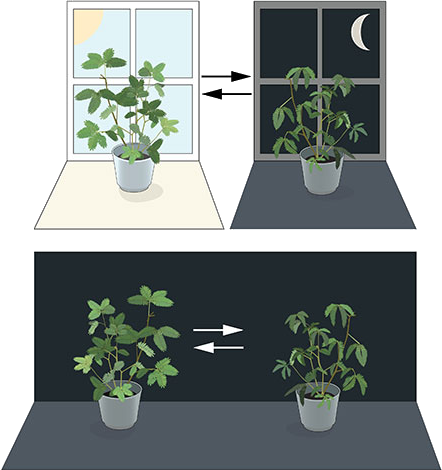
\includegraphics[width=0.6\linewidth,height=\textheight,keepaspectratio]{qmd/images/nobel-prize-outreach-ab-2017-figure-1.png}

\legend{Source: Reproduced from \textcite{nobelprizeoutreachab}.}

}

\end{figure}%

Various biological rhythms have already been shown and described by
science. These rhythms can occur at different description levels,
whether at a higher level, such as the menstrual cycle
\autocite{ecochard2024}, or even at a lower level, such as rhythms
expressed within cells \autocite{buhr2013,sartor2023}. Like many other
biological phenomena, these are emergent properties of complex systems
found in all living beings---stable macroscopic patterns arising from
the collective behavior of the system's parts, resulting in properties
not attainable by the aggregate summation
\autocite{epstein1999,holland2014}. Today, it is understood that
endogenous rhythms provide organisms with an anticipatory capacity,
enabling them to pre-emptively organize resources and activities
\autocite{aschoff1989a}.

Despite the endogenous nature of these rhythms, they can still be
regulated by the external environment. Signals (cues) from the
environment that occur cyclically in nature and have the ability to
regulate biological rhythmic expression are called
zeitgebers\footnote{From the German \emph{zeit}, meaning time, and
  \emph{geber}, meaning donor \autocite{cambridgeuniversitypress}.}.
These zeitgebers act as synchronizers by entraining the phases of the
rhythms \autocite{khalsa2003,minors1991}
(Figure~\ref{fig-chapter-2-kuhlman-2018-figure-2b}). Among the known
zeitgebers are, for example, meal timing \autocite{flanagan2021} and
changes in environmental temperature. However, the most influential of
them is the light/dark cycle (or, simply, light exposure)
\autocite{aschoff1960,pittendrigh1960,roenneberg2016}. It is understood
that the day/night cycle, resulting from the rotation of the Earth, has
provided the vast majority of organisms with an oscillatory system with
a periodic duration of approximately 24 hours
\autocite{aschoff1989a,roenneberg2007}.

\begin{figure}[H]

\caption{\label{fig-chapter-2-kuhlman-2018-figure-2b}Illustration of a
circadian rhythm entrained (Phase-advanced, indicated by a leftward
shift) by a zeitgeber (Input).}

\centering{

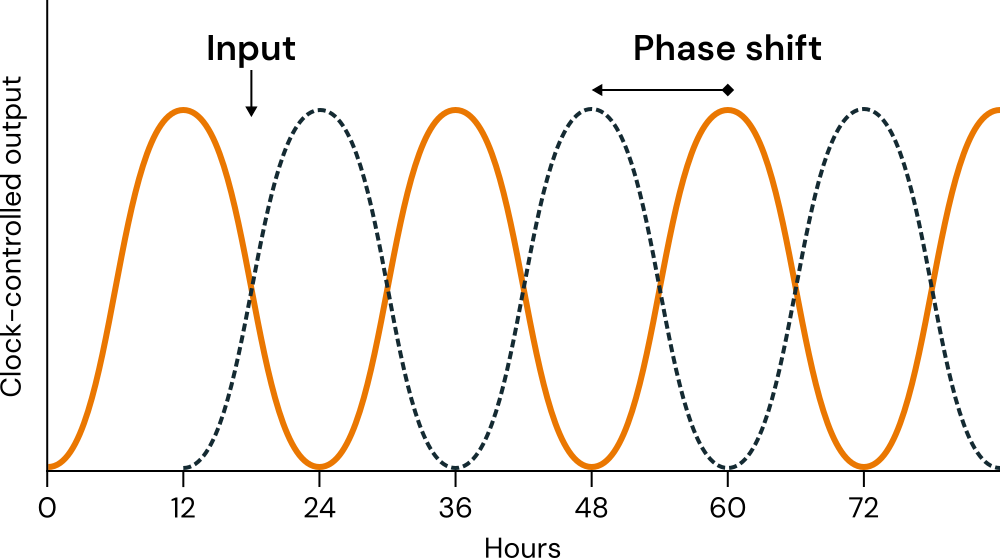
\includegraphics[width=0.85\linewidth,height=\textheight,keepaspectratio]{qmd/images/kuhlman-2018-figure-2b-adapted.png}

\legend{Source: Adapted by the author from \textcite[Figure
2B]{kuhlman2018}.}

}

\end{figure}%

The expression of this temporal organization varies among organisms,
even within the same species (\textcite{duffy2011a};
\textcite{silverio2024}). These variations can be attributed to
differences in how organisms experience their environment or to
differences in their endogenous rhythmicity, a characteristic ultimately
influenced by gene expression \autocite{roenneberg2007a}. The interplay
between environmental influences and genetic predisposition results in
an observable characteristic: the phenotype \autocite{frommlet2016a}.

The various temporal characteristics of an organism can be linked to
different oscillatory periods. Among these are circadian phenotypes,
which refer to characteristics observed in rhythms with periods lasting
about a day \autocite{foster2005a}. Another term used for these temporal
phenotypes, as the name suggests, is \emph{chronotype}
\autocite{ehret1974a,pittendrigh1993}. This term is also often used to
differentiate phenotypes on a spectrum ranging from morningness to
eveningness \autocite{horne1976,roenneberg2019b}.

Sleep is a phenomenon that exhibits circadian expression. By observing
the sleep characteristics of individuals, it is possible to assess the
distribution of circadian phenotypes within a population, thereby
investigating their covariates and other relevant associations
\autocite{roenneberg2003b}. This is because sleep is understood to
result from the interaction of two processes: a homeostatic process (The
\(\text{S}\) process), which is sleep-dependent and accumulates with
sleep deprivation, and a circadian process (The \(\text{C}\) process),
whose expression can be influenced by zeitgebers such as the light/dark
cycle \autocite{borbely1982a,borbely2016a}. These two processes are
illustrated in Figure~\ref{fig-chapter-2-borbely-1982-figure-4}. Because
the circadian rhythm is a component of sleep, its characteristics can be
inferred by isolating its effects from those of the \(\text{S}\)
process.

\begin{figure}[H]

\caption{\label{fig-chapter-2-borbely-1982-figure-4}Illustration of the
interaction between Process \(\text{S}\) (Homeostatic/Sleep-dependent
process) and Process \(\text{C}\) (Circadian rhythm process) in sleep
regulation. \microskip \\ The figure depicts two scenarios: One with
\(17\) hours of wakefulness followed by \(7\) hours of sleep, and
another, under sleep deprivation, with \(41\) hours of wakefulness
followed by \(7\) hours of sleep. The hatched areas indicate periods of
sleep, illustrating the exponential decline of Process \(\text{S}\).}

\centering{

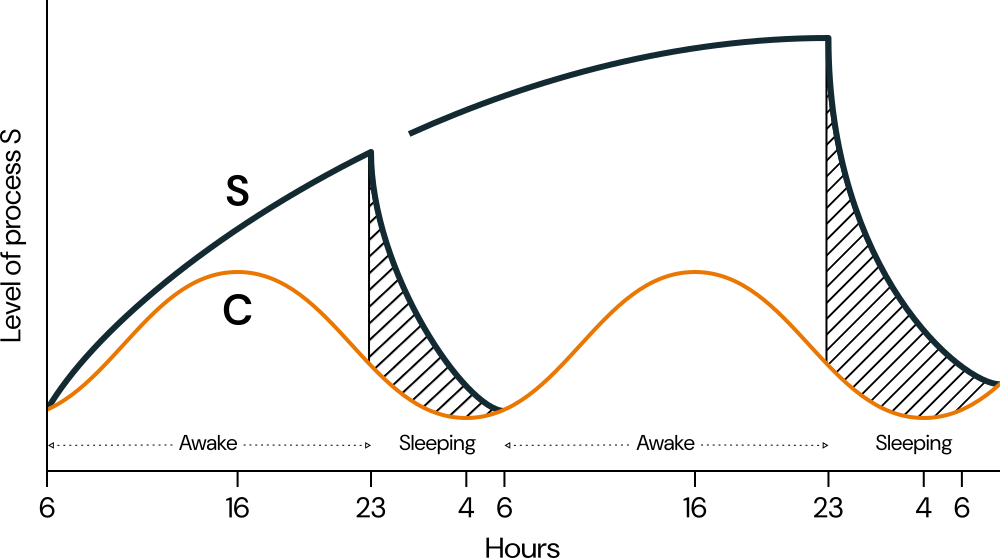
\includegraphics[width=0.85\linewidth,height=\textheight,keepaspectratio]{qmd/images/borbely-1982-figure-4-adapted.png}

\legend{Source: Adapted by the author from \textcite[Figure
4]{borbely1982a}.}

}

\end{figure}%

Building on this idea, \textcite{roenneberg2003b} developed the Munich
Chronotype Questionnaire (MCTQ) to measure the circadian phenotype
through sleep patterns. The MCTQ asks individuals about their sleep
habits, such as the times they go to bed and wake up on workdays and
work-free days. From this information, the MCTQ derives the midpoint of
sleep on work-free days, representing the average of sleep onset and
offset times (Figure~\ref{fig-chapter-2-mctq-variables}). If sleep
deprivation is detected on workdays, the scale adjusts the measurement
accordingly. This midpoint, reflecting sleep under minimal social
constraints, is considered a closer approximation of the intrinsic
circadian rhythm and, therefore, a useful proxy for estimating the
circadian phenotype (the \(\text{C}\) process)
\autocite{leocadio-miguel2014}.

\begin{figure}[H]

\caption{\label{fig-chapter-2-mctq-variables}Variables measured by the
Munich Chronotype Questionnaire (MCTQ). In its standard version, these
variables are collected in the context of workdays and work-free days.
\microskip \\ BT = Local time of going to bed. SPrep = Local time of
preparing to sleep. SLat = Sleep latency (Duration. Time to fall asleep
after preparing to sleep). SO = Local time of sleep onset. SD = Sleep
duration. \textbf{MS} = Local time of mid-sleep. SE = Local time of
sleep end. Alarm = Indicates whether the respondent uses an alarm clock.
SI = ``Sleep inertia'' (Duration. Despite the name, this variable
represents the time the respondent takes to get up after sleep end). GU
= Local time of getting out of bed. TBT = Total time in bed.}

\centering{

\pandocbounded{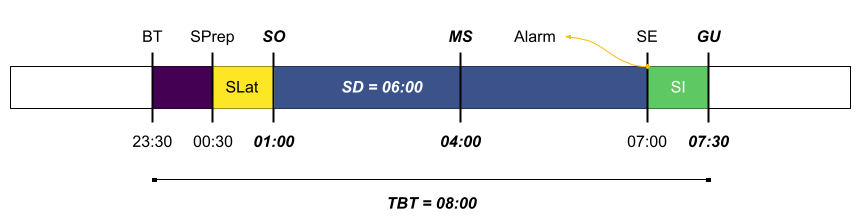
\includegraphics[keepaspectratio]{qmd/images/mctq-figure-1.png}}

\legend{Source: Created by the author.}

}

\end{figure}%

The MCTQ facilitates the evaluation of chronotype in population studies.
This thesis employs the MCTQ to assess chronotype using data from a 2017
online survey conducted by the author, which includes responses from
\(65,824\) Brazilians and geographical information such as postal codes.
This dataset enables the investigation of potential associations between
chronotype and geographic factors.

\bookmarksetup{startatroot}

\chapter{On Complexity Science}\label{sec-on-complexity-science}

Complexity science is the science dedicated to understanding emergent
phenomena \autocite{krakauer2024}. Like computer science and
chronobiology, it began to take shape in the second half of the 20th
century\footnote{Brian Castellani \& Lasse Gerrits created a visual map
  to illustrate the different fields and components of complexity
  science. You can find it at
  \url{https://www.art-sciencefactory.com/complexity-map_feb09.html}.},
by the convergence of several fields, such as systems theory, game
theory, and nonlinear dynamics \autocite{sayama2015}.

At a fundamental level, emergence can be defined as stable macroscopic
patterns arising from local interactions \autocite{epstein1999}. These
patterns emerge from the collective actions of a system's parts, which
cannot be attained by simply summing them up \autocite{holland2014}
(Figure~\ref{fig-chapter-3-lewin-1993-figure-1}). They may give rise to
new properties in a system, which can only be studied by observing the
interactions within it.

\begin{figure}[H]

\caption{\label{fig-chapter-3-lewin-1993-figure-1}An illustration of the
reciprocal action between an emergent phenomenon derived by local
interactions.}

\centering{

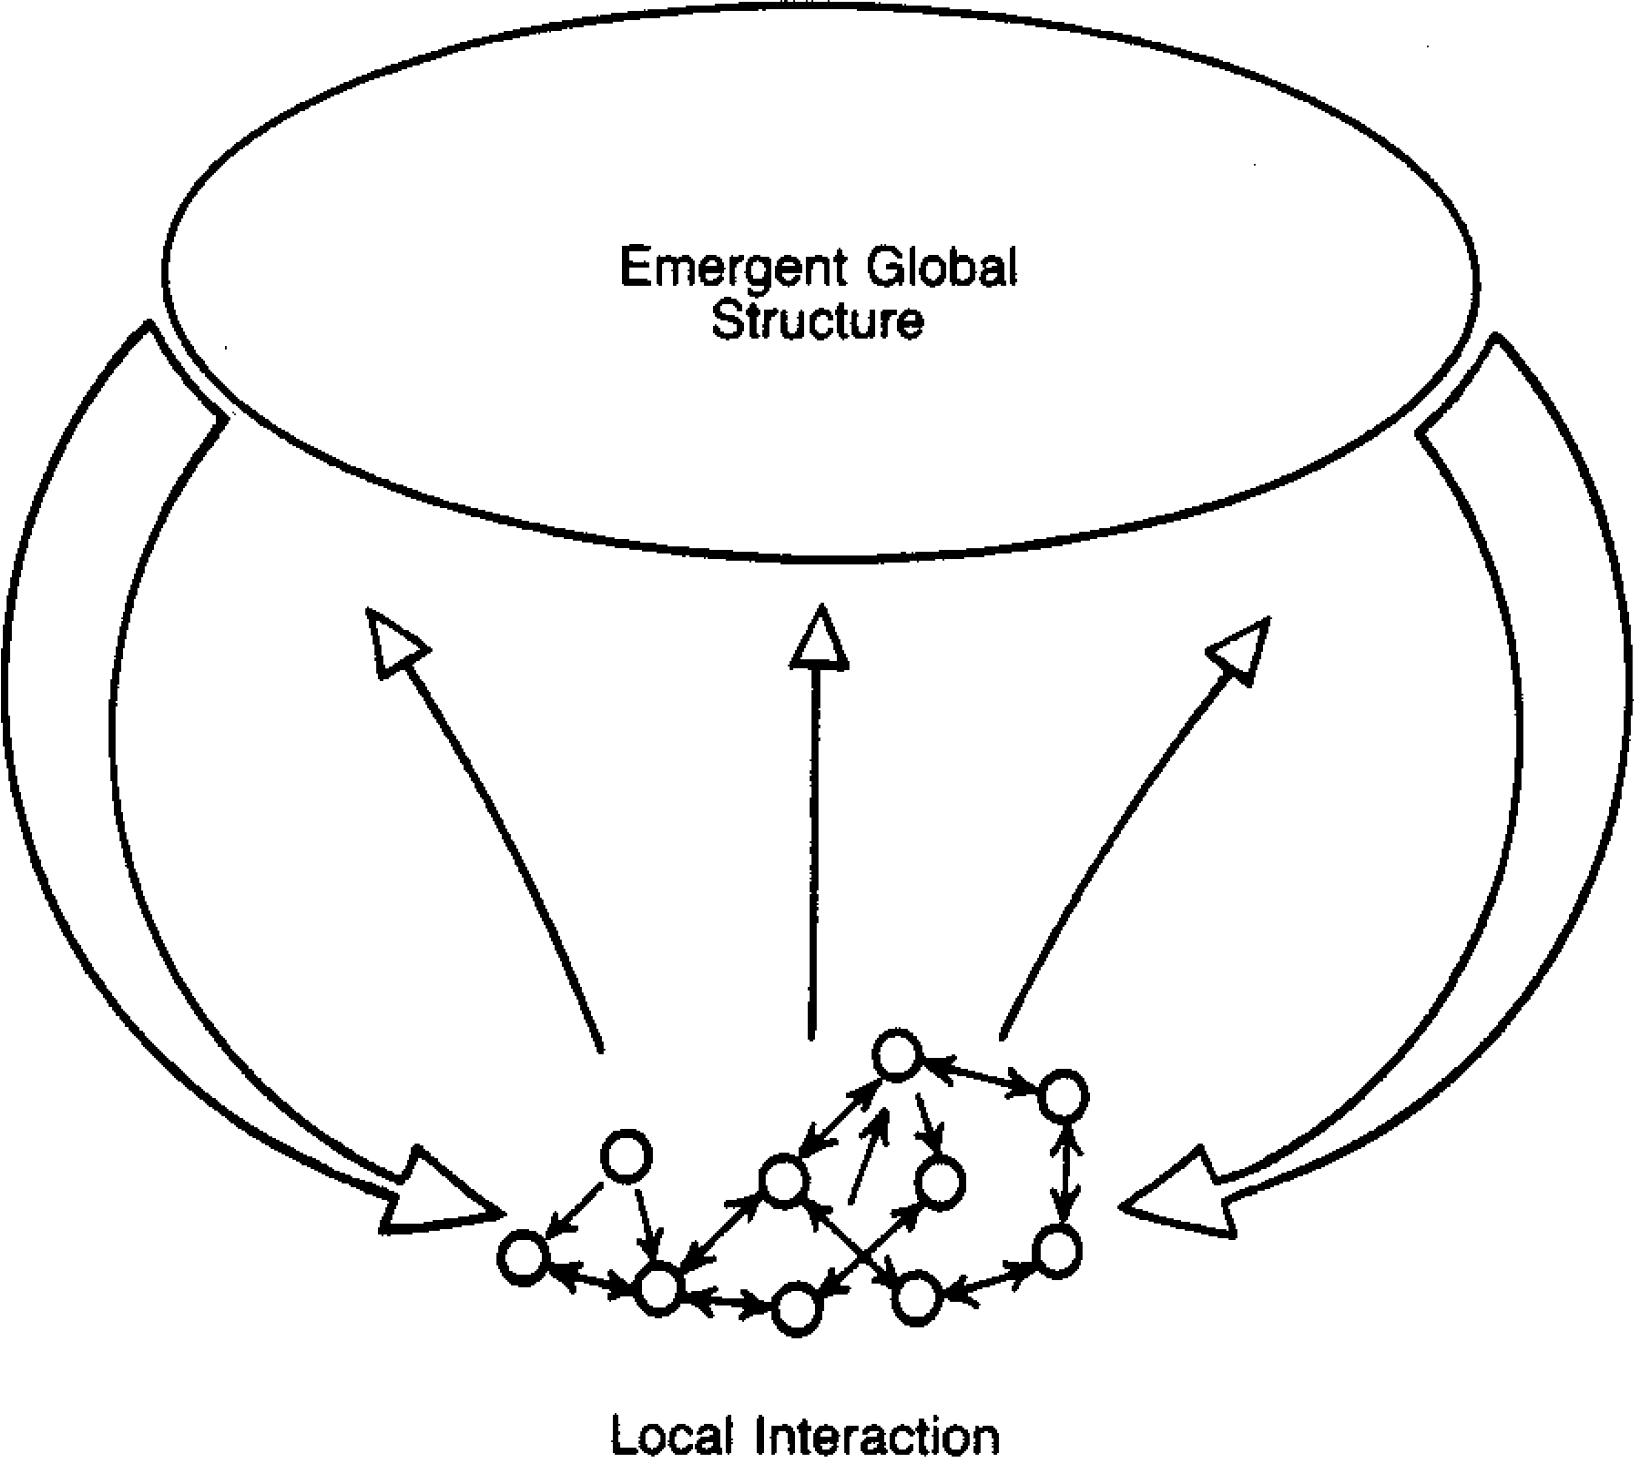
\includegraphics[width=0.65\linewidth,height=\textheight,keepaspectratio]{qmd/images/lewin-1993-figure-1.png}

\legend{Source: Reproduced from \textcite[Figure 1]{lewin1993}.}

}

\end{figure}%

Systems that exhibit emergent properties are considered complex systems
\autocite{mitchell2009a,holland2014}. In a general sense, a system can
be defined as a set of interacting parts that, through their
interactions, produce a global behavior \autocite{vonbertalanffy1968}.
While both complicated and complex systems consist of many interacting
parts, the defining characteristic of complex systems is that they
cannot be fully understood by analyzing their components in isolation
\autocite{holland1992b}. This distinction poses significant challenges,
as traditional methods for studying systems are often inadequate for
capturing the intricate dynamics of complex systems
\autocite{holland2006}.

Biological rhythms are an example of emergent properties produced by a
complex system with multiple levels of interaction
\autocite{partch2014}. Molecular oscillations are generated at the
cellular level \autocite{merrow2005,buhr2013}. These oscillations
interact and couple with one another, forming a complex circadian
network that coordinates rhythmic physiology and behavior
\autocite{raj2008,foster2020}. Although science has not fully mapped all
the pathways, it is understood that in this kaleidoscopic array of
simultaneous interactions, a global rhythm emerges. Each rhythm, or
clock, is itself an emergent phenomenon, interacting with others to
produce a global behavior
(Figure~\ref{fig-chapter-3-flanagan-2021-figure-2}). As the parts
generate these emergences, the emergent feedback to the parts,
regulating and modulating functions at all levels
\autocite{roenneberg2007}.

\begin{figure}[H]

\caption{\label{fig-chapter-3-flanagan-2021-figure-2}An illustration
depicting how the human circadian clock system regulate multiple aspects
of metabolic physiology, such as: hormone secretion, core body
temperature, resting metabolic rate, and plasma metabolite
concentration.}

\centering{

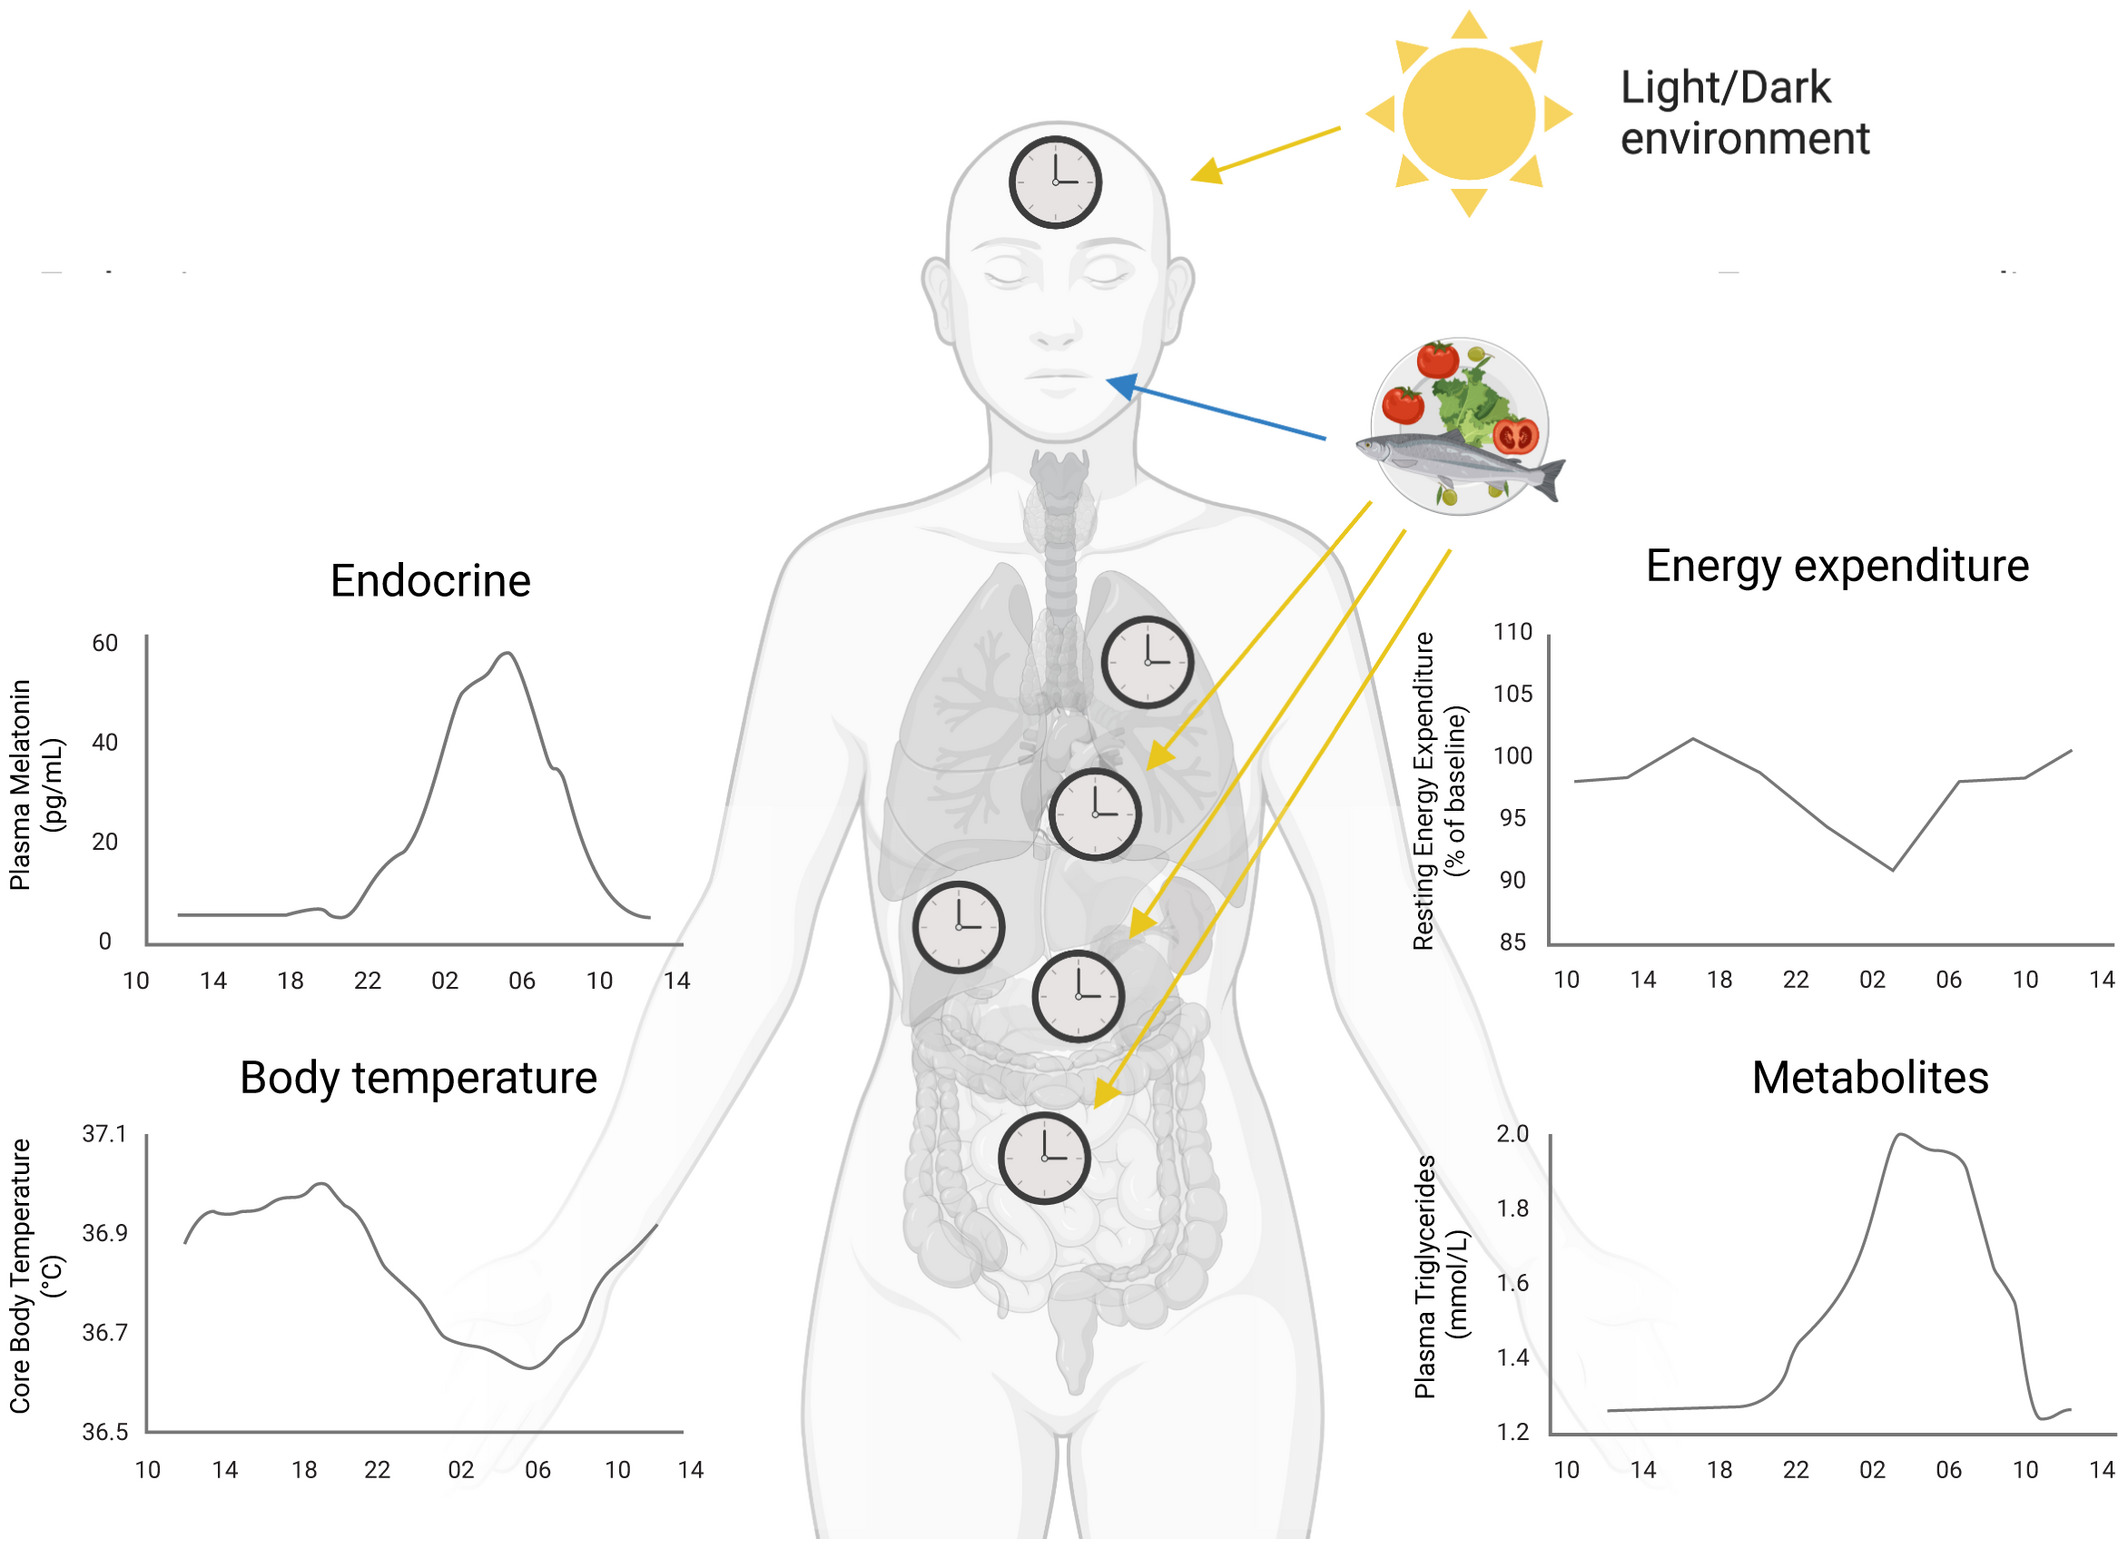
\includegraphics[width=0.85\linewidth,height=\textheight,keepaspectratio]{qmd/images/flanagan-2021-figure-2.png}

\legend{Source: Reproduced from \textcite[Figure 2]{flanagan2021}.}

}

\end{figure}%

The entrainment of these rhythms with environmental periodicities can
involve different mechanisms. For the light/dark cycle, the main
zeitgeber, this involves a network of photosensitive retinal ganglion
cells (pRGCs) that send signals to the suprachiasmatic nucleus (SCN) in
the hypothalamus \autocite{brainard2001,thapan2001}. The SCN then sends
signals to the pineal gland, which produces melatonin, a hormone that
regulates sleep-wake cycles, among other functions
\autocite{foster2021a}.

To model this phenomenon, one must understand how complex systems behave
and can be studied. This thesis adopts a global approach to
understanding the effect of light/dark cycle entrainment on circadian
expressions of populations, considering potential interactions for
proper system control. Given the thesis's aim to test the latitude
hypothesis, a global approach is appropriate. Alternatively, a local
approach could explore entrainment in populations by modeling
individuals, each with their own circadian clock, and their interactions
with the environment.

\bookmarksetup{startatroot}

\chapter{On the Latitude
Hypothesis}\label{sec-on-the-latitude-hypothesis}

The first mention of this hypothesis regarding human populations dates
back to at least 1973 \autocite{bohlen1973}, with earlier hints of the
idea coming from Erhard Haus and Franz Halberg in 1970
\autocite[101]{haus1970}, building on discussions initiated by Jürgen
Aschoff \autocite{aschoff1969}. Since then, numerous studies have
explored this topic, yielding somewhat conflicting results\footnote{A
  systematic review on the subject is provided by
  \textcite{randler2017}.}.

The hypothesis, also called the environment hypothesis
\autocite{horzum2015}, posits that regions closer to the poles receive,
on average, less annual sunlight compared to regions near the equator
(Figure~\ref{fig-chapter-4-hut-2013-figure-1}). Consequently, regions
around latitude \(0°\) are thought to have a stronger solar zeitgeber.
According to chronobiological theories, this stronger zeitgeber would
enhance the entrainment of circadian rhythms with the light/dark cycle,
resulting in lower variability of circadian phenotypes
(\textcite{aschoff1960}; \textcite{pittendrigh1960}
\textcite{aschoff1981}; \textcite{pittendrigh1989};
\textcite{pittendrigh1991}). This reduced influence of individual
endogenous periods is illustrated in
Figure~\ref{fig-chapter-4-roenneberg-2003-figure-7-f-adapted}.

\begin{figure}[H]

\caption{\label{fig-chapter-4-hut-2013-figure-1}Annual variations in (a)
Twilight duration, (b) Photoperiod, and (c) Temperature across different
latitudes. Each color represents a specific latitude.}

\centering{

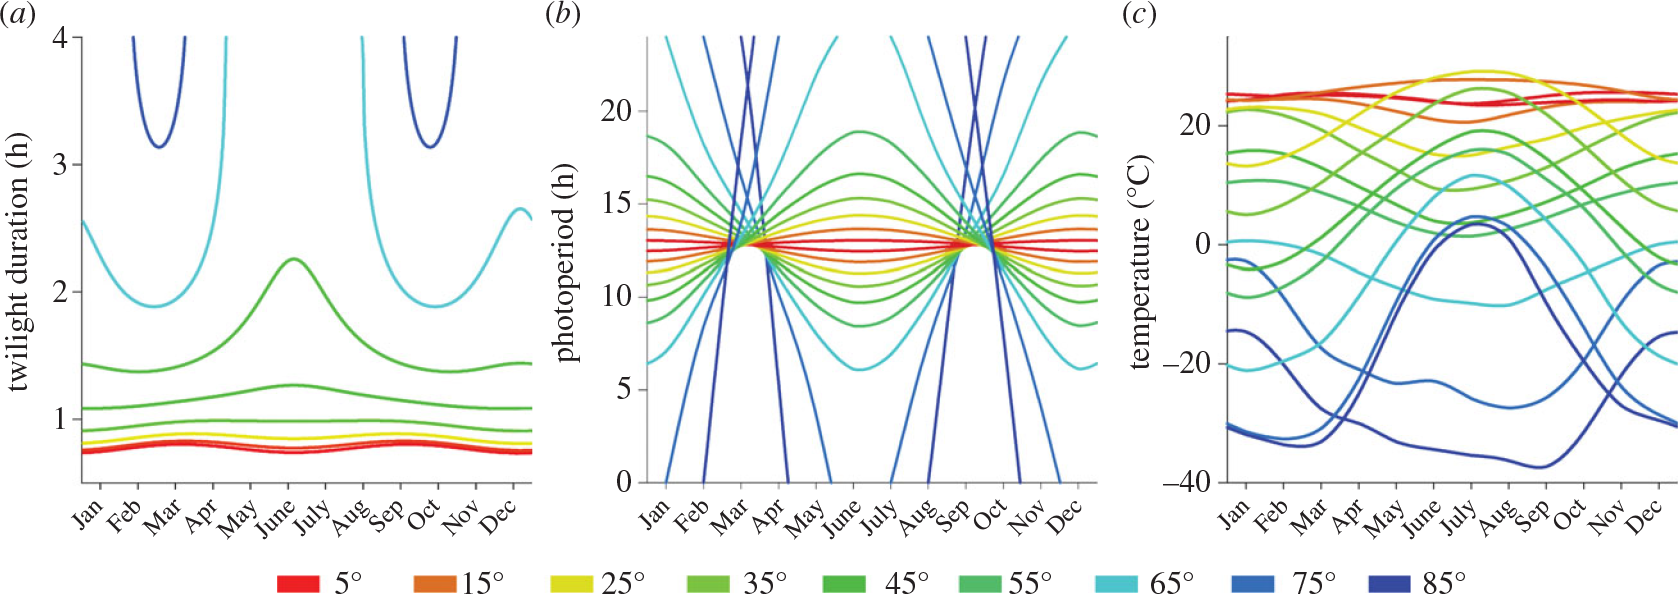
\includegraphics[width=1\linewidth,height=\textheight,keepaspectratio]{qmd/images/hut-2013-figure-1.png}

\legend{Source: Reproduced from \textcite[Figure 1]{hut2013}.}

}

\end{figure}%

In contrast, populations near the poles would experience a weaker solar
zeitgeber, leading to greater variability for the expression of
circadian phenotypes. This disparity also would translate into
differences in mean chronotype: Equatorial populations would tend to
exhibit a morningness orientation, while populations at higher and low
latitudes would tend toward eveningness
\autocite{bohlen1973,roenneberg2003b}.

It's important to emphasize that the latitude hypothesis is grounded in
underlying circadian rhythms, not in self-reported
morningness-eveningness (ME) \emph{preference}. Self-reported preference
can be influenced by extraneous factors, such as social constraints.
Reducing this hypothesis to individual preferences undermines its
theoretical foundation and introduces unnecessary confounders.
Therefore, chronotype scales focusing on the preference aspect of ME may
be unsuitable for testing this hypothesis. This is illustrated by
\textcite{leocadio-miguel2014} when discussing differences between the
Horne-Östberg (HO) ME questionnaire \autocite{horne1976}, which treats
chronotype as a psychological construct \autocite{roenneberg2019c}, and
the Munich Chronotype Questionnaire \autocite{roenneberg2003b}, which
addresses chronotype as a biological construct, in the context of the
latitude hypothesis.

\begin{figure}[H]

\caption{\label{fig-chapter-4-roenneberg-2003-figure-7-f-adapted}Chronotype
distributions under the influence of strong (orange) and weak (black)
zeitgebers. This visualization reflects the effect proposed by the
latitude hypothesis.}

\centering{

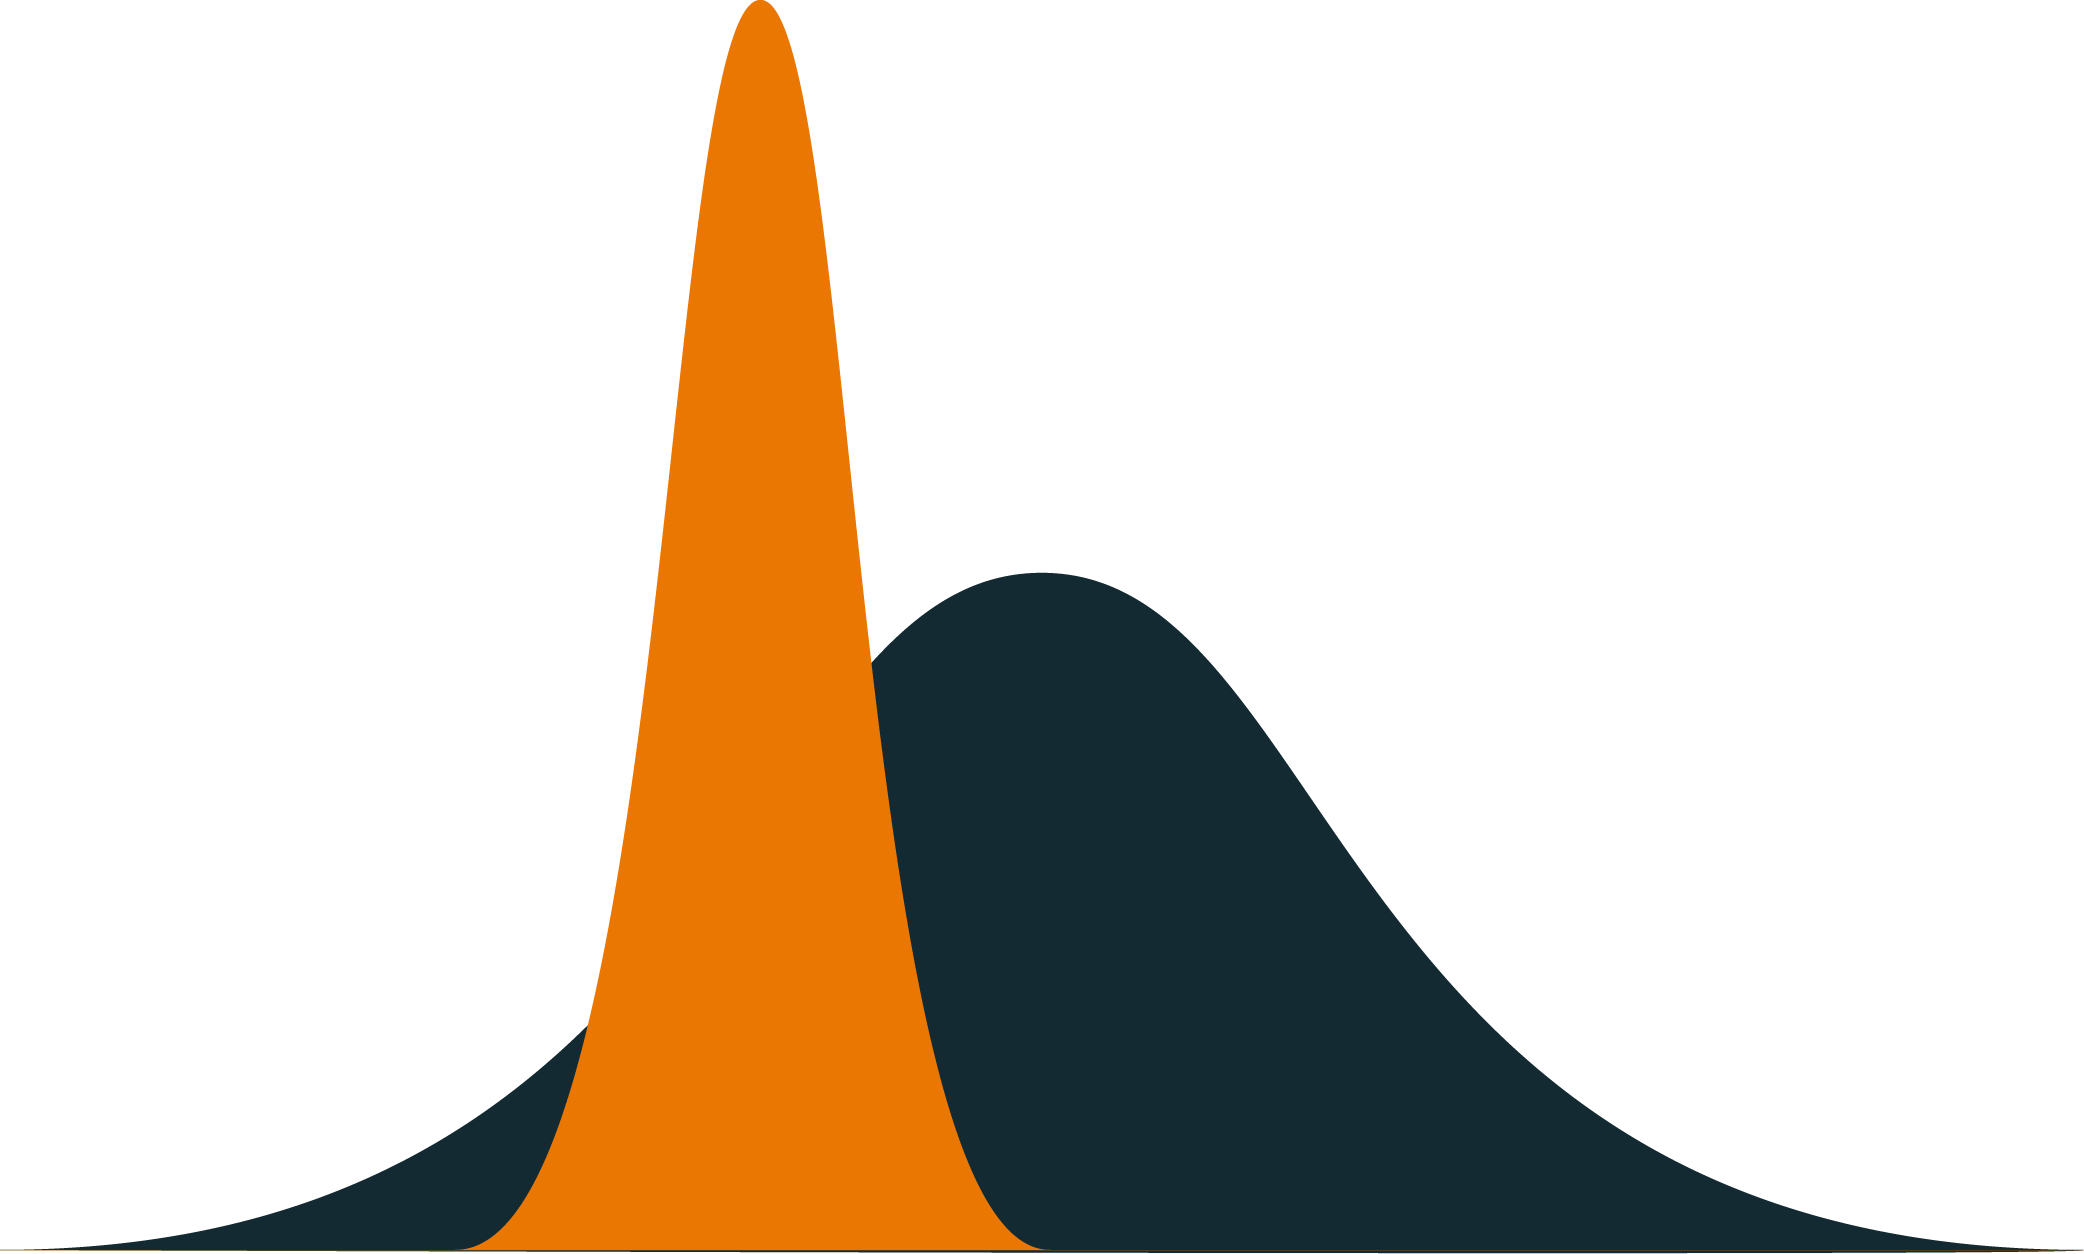
\includegraphics[width=0.75\linewidth,height=\textheight,keepaspectratio]{qmd/images/roenneberg-2003-figure-7-f-adapted.png}

\legend{Source: Adapted by the author from \\ \textcite[Figure
7F]{roenneberg2003b}.}

}

\end{figure}%

While there is some compelling evidence for this hypothesis in some
insect species \autocite{hut2013}, the same cannot be said for this
association in humans. Some authors claim to found such an association
(\textcite{randler2008}; \textcite{leocadio-miguel2014};
\textcite{horzum2015}; \textcite{leocadio-miguel2017};
\textcite{wang2023}), but a closer look at the data reveals that the
evidence is not as clear as it seems.

For example, \textcite{leocadio-miguel2017} claimed to find a meaningful
association between latitude and chronotype in a sample of \(12,884\)
Brazilian participants using the HO questionnaire. However, the reported
effect size was too small to be considered practically significant (even
by lenient standards), with latitude explaining only approximately
\(0.388\%\) of the variance in chronotype (Cohen's
\(f^2 = 0.004143174\))
(Figure~\ref{fig-chapter-4-leocadio-miguel-2017-figure-2}) (See the
Supplemental Materials for an in-depth analysis of this result).
Considering the particular emphasis that the solar zeitgeber has on the
entrainment of biological rhythms (as demonstrated by numerous studies),
it is unreasonable to assume that the latitude hypothesis could be
supported without at least a non-negligible effect size.

The results from the latitude hypothesis highlight common limitations of
studies relying on Null Hypothesis Significance Testing (NHST). A
\emph{p}-value does not measure effect size; rather, it represents the
conditional probability of observing the test statistic (or a more
extreme value) given that the null hypothesis is true
\autocite{cohen1994,wasserstein2016}. As \textcite[16]{cohen1988a}
noted, the goal in NHST is not to test whether the population effect
size is literally zero, but rather whether it is negligible or trivial.

\begin{figure}[H]

\caption{\label{fig-chapter-4-leocadio-miguel-2017-figure-2}Mean scores
(±SE) on the Horne \& Östberg (HO) chronotype scale \autocite{horne1976}
across a latitudinal gradient, along with corresponding annual average
solar irradiation levels (W/m²). \microskip \\ The HO scale comprises 19
items, with total scores ranging from 16 to 86; lower scores indicate a
stronger evening orientation, while higher scores reflect a greater
morning orientation. Notably, the y-axis exaggerates the visual impact
of the differences, as it spans a range of only approximately \(4\)
points, which overstate the perceived significance of the effect.}

\centering{

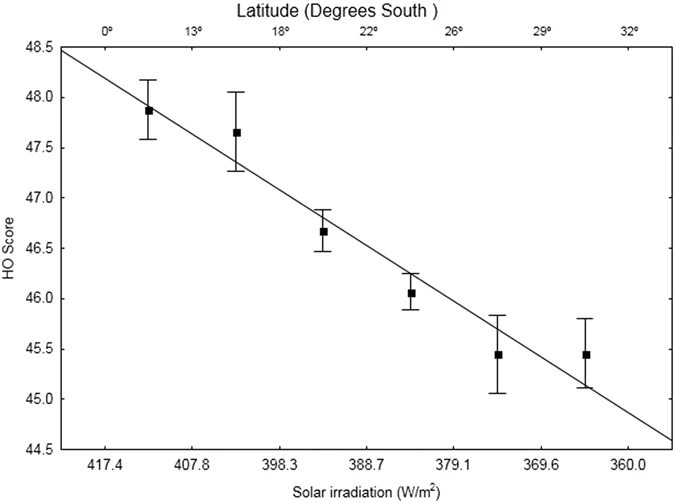
\includegraphics[width=0.8\linewidth,height=\textheight,keepaspectratio]{qmd/images/leocadio-miguel-2017-figure-2.png}

\legend{Source: Reproduced from \textcite[Figure
2]{leocadio-miguel2017}.}

}

\end{figure}%

Several factors may undermine this hypothesis, such as selective light
exposure and social constraints \autocite{skeldon2021}. To gain a more
accurate understanding of the mechanisms underlying chronotype
expression, it remains crucial to test this hypothesis in larger samples
and with robust statistical procedures. This study aims to address this
gap.

\newpage

\null\vfill

\begingroup
\hyphenpenalty=100000
\noindent The following study was designed for publication in the journal \href{https://www.nature.com/srep/}{\textit{Scientific Reports}} (\href{https://jcr.clarivate.com/jcr}{IF 2023: 3.8/JCR} | \href{https://sucupira-legado.capes.gov.br/sucupira/}{CAPES: A1/2017-2020}) and structured in accordance with the journal's \href{https://www.nature.com/srep/author-instructions/submission-guidelines}{submission guidelines}.
\endgroup

\vspace{\hugeskipamount}

\bookmarksetup{startatroot}

\chapter{Is Latitude Associated with
Chronotype?}\label{sec-latitude-hypothesis-article}

\section{Abstract}\label{abstract}

\noindent \textbf{Chronotypes are temporal phenotypes that reflect our
internal temporal organization, a product of evolutionary pressures
enabling organisms to anticipate events. These intrinsic rhythms are
entrain by zeitgebers---periodical environmental stimuli with the
ability to regulate biological rhythmic expression, with light exposure
being the primary mechanism. Given light's role in these systems,
previous research hypothesized that latitude might significantly
influence chronotypes, suggesting that populations near the equator
would exhibit more morning-leaning characteristics due to more
consistent light/dark cycles, while populations near the poles might
display more evening-leaning tendencies with a potentially freer
expression of intrinsic rhythms. To test this hypothesis, we analyzed
chronotype data from a large sample of \(65,824\) subjects across
diverse latitudes in Brazil. Our results revealed a negligeble effect
size of latitude on chronotype
(\(f^2 = 0.00314, 95\% \ \text{CI}[0, 0.0122]\)), indicating that the
entrainment phenomenon is far more complex than previously conceived.
These findings challenge simplified environmental models of biological
timing and underscore the need for more nuanced investigations into the
mechanisms underlying temporal phenotypes, opening new avenues for
understanding the intricate relationship between environmental cues and
individual circadian rhythms.}

\section{Introduction}\label{introduction}

Humans exhibit a variety of observable traits, such as eye or hair
color, which are referred to as phenotypes. These phenotypes also
manifest in the way our bodies function.

A chronotype is a temporal phenotype
\autocite{ehret1974a,pittendrigh1993}, typically used to refer to
endogenous circadian rhythms---biological rhythms with periods close to
24 hours. Chronobiology, the science that studies biological rhythms,
suggests that the evolution of these internal oscillators is closely
linked to our environment, particularly to the day/night cycle. Is
believed that this cycle, alongside human evolution, created
environmental pressures that led to the development of temporal
organization within organisms
\autocite{pittendrigh1981,aschoff1989,paranjpe2005}. Such organization
allowed organisms to predict events and better manage their needs, such
as storing food for winter \autocite{aschoff1989a}.

For a temporal system to be effective, it must adapt to environmental
changes. Environmental cues that regulate biological rhythms are termed
zeitgebers (from the German \emph{zeit}, meaning time, and \emph{geber},
meaning giver \autocite{cambridgeuniversitypress}). These zeitgebers act
as inputs that shift and synchronize biological rhythms through a
process known as entrainment \autocite{khalsa2003,minors1991}.

The primary zeitgeber influencing biological rhythms is the light/dark
cycle, or, simply, light exposure
\autocite{aschoff1960,pittendrigh1960,roenneberg2016}. Given its
significant role in entraining the biological clock, several studies
have hypothesized that the latitudinal shift of the sun, due to the
Earth's axial tilt, might lead to different temporal traits in
populations near the equator compared to those closer to the poles
\autocite{bohlen1973,randler2008,leocadio-miguel2014,horzum2015,leocadio-miguel2017}.
This is based on the idea that populations at low or higher latitudes
experience greater fluctuations in sunlight and a weaker overall solar
zeitgeber. This concept is known as the latitude hypothesis, or the
environmental hypothesis of circadian rhythm regulation.

Several studies have claimed to find this association in humans, but the
evidence they provide is of very low quality or simply misleading
\autocites[e.g.,][]{randler2008,leocadio-miguel2014,horzum2015,leocadio-miguel2017,wang2023}.
A notable attempt was made by \textcite{leocadio-miguel2017}, who
measured the chronotype of \(12,884\) Brazilian subjects across a wide
latitudinal range using the Horne-Östberg (HO) Morningness--Eveningness
questionnaire \autocite{horne1976}. Although the authors concluded that
there was a meaningful association between latitude and chronotype,
their results were too small to be considered practically significant
(even by lenient standards), with latitude explaining only approximately
\(0.388\%\) of the variance in chronotype (Cohen's \(f^2 = 0.00414\)).
One possible explanation for this result is that the HO measures
psychological traits rather than the biological states of circadian
rhythms themselves \autocite{roenneberg2019c}, suggesting it may not be
the most suitable tool for testing the hypothesis
\autocite{leocadio-miguel2014}.

Building on \textcite{leocadio-miguel2017}, this study offers a novel
attempt to test the latitude hypothesis by employing a biological
approach through the Munich ChronoType Questionnaire (MCTQ)
\autocite{roenneberg2003b} and an enhanced statistical methodology.
Additionally, it utilizes the largest dataset on chronotype from a
single country, as far as the existing literature suggests, comprising
\(65,824\) respondents, all residing within the same timezone in Brazil
and completing the survey within a one-week window
(Figure~\ref{fig-chapter-5-sample-geographical-distribution}).

\begin{figure}[H]

\caption{\label{fig-chapter-5-sample-geographical-distribution}Geographical
distribution of the sample used in the analysis (\(n = 65,824\)).
\microskip \\ Each point represents a municipality, with its size
proportional to the number of participants and color intensity
increasing with participant count. The sample includes Brazilian
individuals aged 18 or older, residing in the UTC-3 timezone, who
completed the survey between October 15th and 21st, 2017. The size and
color scale are logarithmic (\(\log_{10}\)).}

\centering{

\pandocbounded{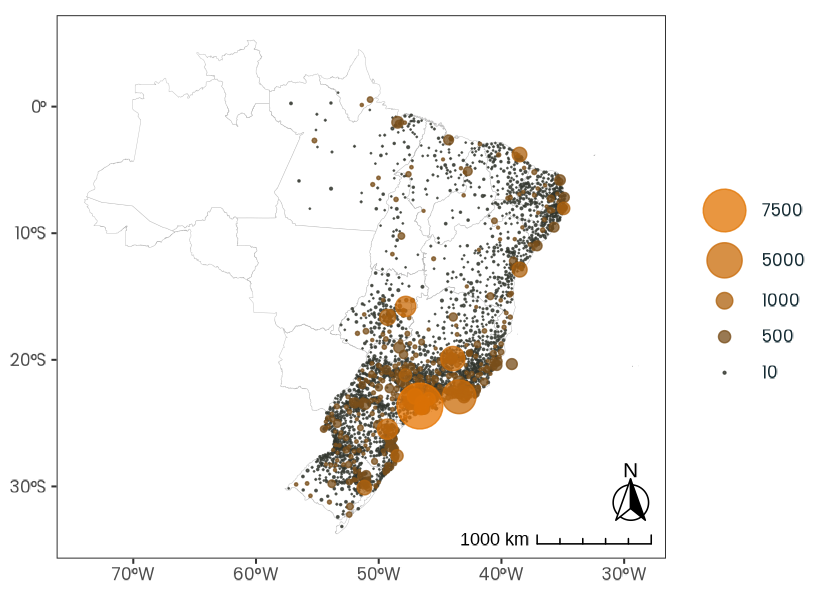
\includegraphics[keepaspectratio]{qmd/chapter-5_files/figure-pdf/unnamed-chunk-5-1.png}}

\legend{Source: Created by the author.}

}

\end{figure}%

\section{Results}\label{results}

The Munich Chronotype Questionnaire (MCTQ) uses the midpoint between
sleep onset (SO) and sleep end (SE) on work-free days
(MSF\textsubscript{sc}), with a sleep correction (sc) applied if sleep
debt is detected, as a proxy for chronotype \autocite{roenneberg2003b}.
For example, if an individual sleeps from \(\text{00:00}\) to
\(\text{08:00}\), the midpoint would be \(\text{04:00}\). This measure
is based on the current understanding of sleep regulation, which
comprises a homeostatic/sleep-dependent process (\(\text{S}\) process)
and a circadian process (\(\text{C}\) process)
\autocite{borbely1982a,borbely2016a}. The midpoint of sleep on free days
offers a way to observe unrestrained sleep behavior, thereby minimizing
the influence of the \(\text{S}\) process and providing a better
approximation of the circadian phenotype (i.e., the \(\text{C}\)
process).

Our analysis revealed an overall mean MSF\textsubscript{sc} of
\(\text{04:28:41}\), with an standard deviation of \(\text{01:26:13}\).
The distribution is shown in
Figure~\ref{fig-chapter-5-chronotype-distribution}.

\begin{figure}[H]

\caption{\label{fig-chapter-5-chronotype-distribution}Observed
distribution of the local time of the sleep-corrected midpoint between
sleep onset and sleep end on work-free days (MSF\textsubscript{sc}), a
proxy for chronotype. \microskip \\ Chronotypes are categorized into
quantiles, ranging from extremely early (\(0 |- 0.11\)) to extremely
late (\(0.88 - 1\)).}

\centering{

\pandocbounded{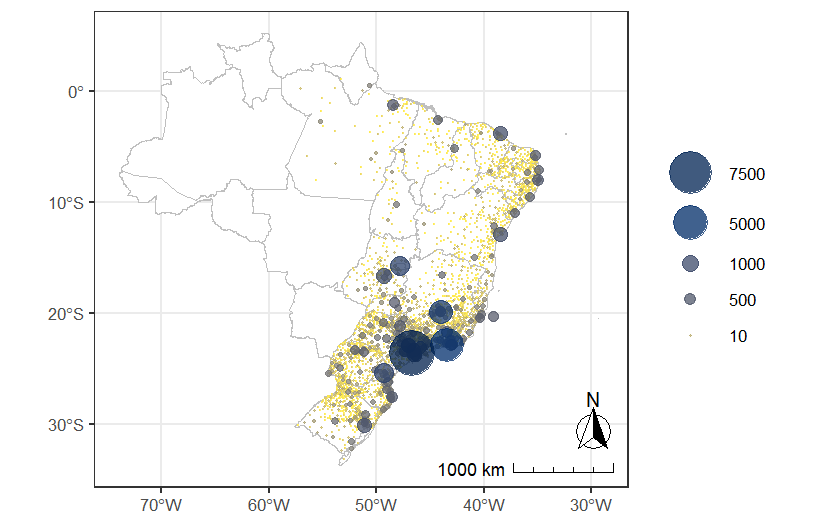
\includegraphics[keepaspectratio]{qmd/chapter-5_files/figure-pdf/unnamed-chunk-6-1.png}}

\legend{Source: Created by the author based on a data visualization from
\\ \textcite[Figure 1]{roenneberg2019b}.}

}

\end{figure}%

This represents the midsleep point for Brazilian subjects living in the
UTC-3 timezone, with an intermediate or average chronotype. Considering
the \(7–9\) hours of sleep recommended for healthy adults by the
American Academy of Sleep Medicine (AASM) \autocite{watson2015b}, one
might infer that this average individual, in the absence of social
constraints, would typically wake up at approximately
\(\text{08:28:41}\).

The study hypothesis was tested using nested multiple regressions, based
on the design of the models presented in \textcite{leocadio-miguel2017}.
The core idea of nested models is to evaluate the effect of including
one or more predictors on the model's variance explanation
(\(\text{R}^2\)) \autocite{maxwell2018}. This is achieved by comparing a
restricted model (without the latitude) with a full model (with the
latitude). Cell weights, based on sex, age group, and state of
residence, were applied to account for sample imbalances.

To ensure practical significance, the hypothesis test incorporated a
minimum effect size (MES) criterion, aligning with the original
Neyman-Pearson framework for data testing
\autocite{neyman1928,neyman1928a,perezgonzalez2015}. The MES was set at
a Cohen's \(f^2\) of \(0.02\) (equivalent to an \(\text{R}^2\) of
\(0.01960784\)), a lenient threshold \autocite{cohen1988a}. Given the
well-established influence of the solar zeitgeber on biological rhythm
entrainment, it is unlikely that the latitude hypothesis could be
meaningfully supported without demonstrating at least a non-trivial
effect.

Two tests were conducted, both starting with the same restricted model,
which included age, sex, longitude, and the average monthly Global
Horizontal Irradiance (GHI) at the time of questionnaire completion as
predictors related to the latitude/longitude of each respondent as
predictors (\(\text{R}^2_{\text{adj}} = 0.08517\),
\(\text{F}(4, 65818) = 1531.808\), \(p\text{-value} < 1e-05\)). The
first full model (\textbf{A}) added the average annual GHI and daylight
duration for the nearest March equinox, as well as the June and December
solstices, as proxies for latitude, following the methods of
\textcite{leocadio-miguel2017} (\(\text{R}^2_{\text{adj}} = 0.08803\),
\(\text{F}(8, 65814) = 794.12\), \(p\text{-value} < 1e-05\)). The second
full model (\textbf{B}) added only latitude as a predictor
(\(\text{R}^2_{\text{adj}} = 0.08568\),
\(\text{F}(5, 65817) = 1233.588\), \(p\text{-value} < 1e-05\)). All
coefficients were statistically different from zero
(\(p\text{-value} < 0.05\)). Assumption checking and residual
diagnostics primarily relied on visual inspection, as formal assumption
tests (e.g., Anderson-Darling) are often not recommended for large
samples \autocite{shatz2024}. All validity assumptions were met, and no
serious multicollinearity was found among the predictor variables.

Sunrise times for the nearest March and September equinoxes, as well as
the June and December solstices, were excluded due to high
multicollinearity. Daylight duration for the September equinox was
excluded for its collinearity with daylight duration during the March
equinox.

An ANOVA for nested models revealed a significant reduction in the
residual sum of squares in both tests (\textbf{A}
\(\text{F}(4, 65814) = 51.71\), \(p\text{-value} < 1e-05\)) (\textbf{B}
\(\text{F}(1, 65817) = 37.325\), \(p\text{-value} < 1e-05\)). However,
similarly to \textcite{leocadio-miguel2017}, when estimating Cohen's
\(f^2\) effect size, the results were below the MES (i.e., negligible)
(\textbf{A} \(f^2 = 0.00314, 95\% \ \text{CI}[0, 0.0122]\)) (\textbf{B}
\(f^2 = 0.00057, 95\% \ \text{CI}[0, 0.00954]\)).

\section{Discussion}\label{discussion}

We emphasize that the assumption of a causal, linear relationship
between latitude and chronotype constitutes an \emph{a priori}
hypothesis, which this study seeks to falsify.

Despite a broad latitudinal range (\(33.85026\) degrees) and a large,
balanced sample, our results indicate that the effect of latitude on
chronotype is negligible. Indeed, despite suggestions of a potential
link in several studies, robust empirical evidence supporting this claim
in humans is lacking.

Our results align with those of \textcite{leocadio-miguel2017}, who
reported a similar effect size (Cohen's \(f^2 = 0.004143174\)). However,
their analysis did not incorporate a minimum effect size criterion,
leading to misleading interpretations.

The small and inconsistent nature of the latitude effect is illustrated
in Figure~\ref{fig-chapter-5-chronotype-latitude-series}, while
Figure~\ref{fig-chapter-5-chronotype-geographical-distribution-by-state}
displays the mean chronotype by Brazilian state. The distribution of
chronotypes across latitudes is further illustrated in
Figure~\ref{fig-chapter-5-chronotype-geographical-distribution-by-respondent}.

\begin{figure}[H]

\caption{\label{fig-chapter-5-chronotype-latitude-series}Boxplots of
observed mean MSF\textsubscript{sc} values aggregated by \(1°\) latitude
intervals, illustrating the relationship between latitude and
chronotype. \microskip \\ MSF\textsubscript{sc} represents the local
time of the sleep-corrected midpoint between sleep onset and sleep end
on work-free days, a proxy for chronotype. Higher MSF\textsubscript{sc}
values indicate later chronotypes. The × symbol points to the mean. The
orange line represents a linear regression. The differences in
mean/median values across latitudes are minimal relative to the Munich
ChronoType Questionnaire (MCTQ) scale.}

\centering{

\pandocbounded{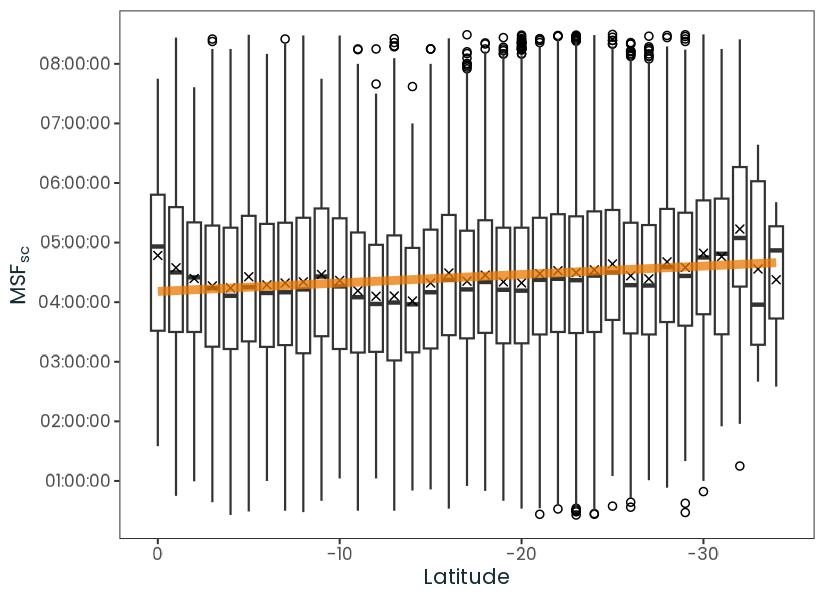
\includegraphics[keepaspectratio]{qmd/chapter-5_files/figure-pdf/unnamed-chunk-7-1.png}}

\legend{Source: Created by the author.}

}

\end{figure}%

The absence of a clear relationship between latitude and chronotype can
be attributed to multiple factors. As Jürgen Aschoff might have put it,
this may reflect a lack of ``ecological significance''
\autocite{aschoff1972}. Even if latitude does influence circadian
rhythms, the effect could be too minor to detect or might be
overshadowed by other, more prominent factors like social behaviors,
work hours, or the widespread use of artificial lighting. Furthermore,
the variations in sunlight exposure between latitudes may not be
substantial enough to meaningfully impact the circadian system, which is
highly responsive to light. Given that even minor light fluctuations can
lead to measurable physiological changes
\autocite{khalsa2003,minors1991}, latitude alone may not be a decisive
factor in determining chronotype.

\begin{figure}[H]

\caption{\label{fig-chapter-5-chronotype-geographical-distribution-by-state}Observed
geographical distribution of MSF\textsubscript{sc} values by Brazilian
state, illustrating how chronotype varies with latitude in Brazil.
\microskip \\ MSF\textsubscript{sc} is a proxy for chronotype,
representing the midpoint of sleep on work-free days, adjusted for sleep
debt. Higher MSF\textsubscript{sc} values correspond to later
chronotypes. The color scale is bounded by the first and third
quartiles. Differences in mean MSF\textsubscript{sc} values across
states are small and fall within a narrow range relative to the scale of
the Munich ChronoType Questionnaire (MCTQ), limiting the significance of
these variations.}

\centering{

\pandocbounded{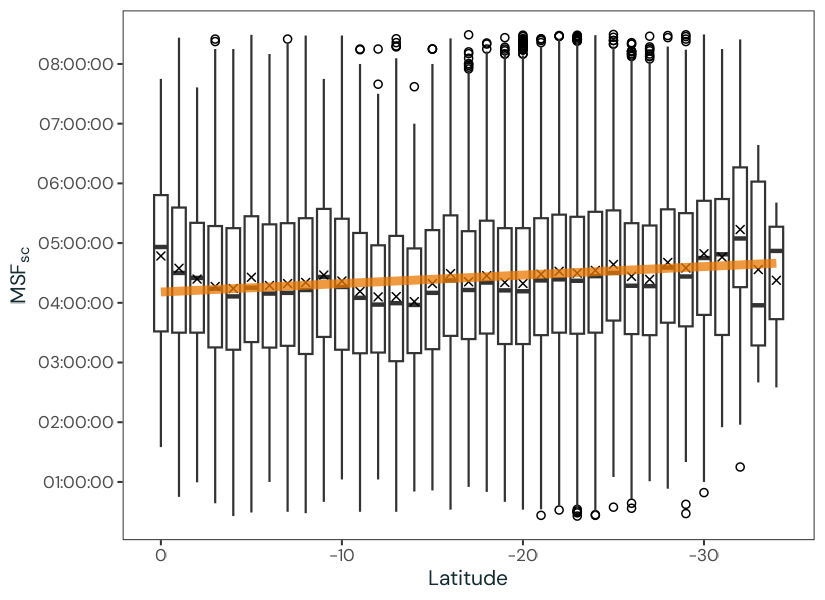
\includegraphics[keepaspectratio]{qmd/chapter-5_files/figure-pdf/unnamed-chunk-8-1.png}}

\legend{Source: Created by the author.}

}

\end{figure}%

The results highlight the complex nature of the human chronotype and
emphasize the importance of investigating alternative factors that may
influence them. The perceived link between these variables may be a
consequence of prioritizing statistical rituals over statistical
thinking and a tendency toward confirmation bias, rather than rigorous
and unbiased data analysis.

\begin{figure}[H]

\caption{\label{fig-chapter-5-chronotype-geographical-distribution-by-respondent}Observed
geographical distribution of MSF\textsubscript{sc} values by a spectrum
of extremely early and extremely late, illustrating how chronotype
varies with latitude in Brazil. \microskip \\ MSF\textsubscript{sc} is a
proxy for chronotype, representing the midpoint of sleep on work-free
days, adjusted for sleep debt. Chronotypes are categorized into
quantiles, ranging from extremely early (\(0 |- 0.11\)) to extremely
late (\(0.88 - 1\)). No discernible pattern emerges from the
distribution of chronotypes across latitudes.}

\centering{

\pandocbounded{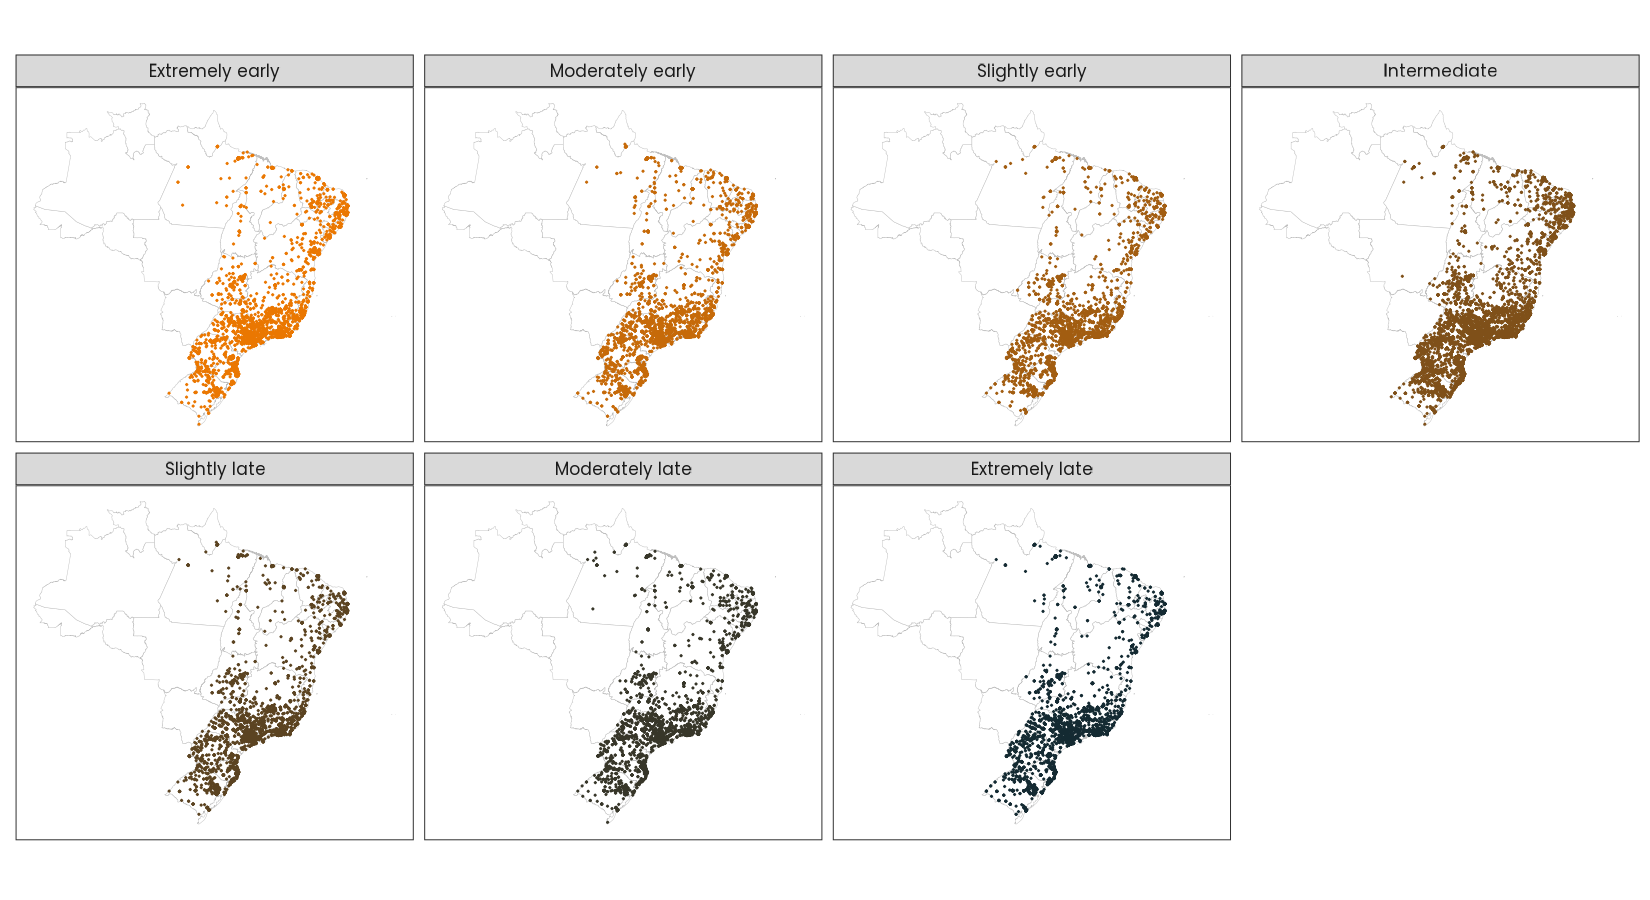
\includegraphics[keepaspectratio]{qmd/chapter-5_files/figure-pdf/unnamed-chunk-9-1.png}}

\legend{Source: Created by the author.}

}

\end{figure}%

While this study does not outright refute the hypothesis, the
association between latitude and chronotype should remain an open
scientific question rather than be treated as established knowledge
until supported by robust evidence.

\section{Methods}\label{methods}

\subsection{Measurement Instrument}\label{measurement-instrument}

Chronotypes were assessed using a sleep log based on the standard
version of the Munich ChronoType Questionnaire (MCTQ)
\autocite{roenneberg2003b}, a well-validated and widely used self-report
tool for measuring sleep-wake behavior and determining chronotype
\autocite{roenneberg2019c}. The MCTQ derives chronotype from the
sleep-corrected midpoint of sleep on free days (MSF\textsubscript{sc}),
which compensates for sleep debt incurred during the workweek
\autocite{roenneberg2012}. Figure~\ref{fig-chapter-5-mctq-variables}
illustrates the variables collected by the MCTQ.

\begin{figure}[H]

\caption{\label{fig-chapter-5-mctq-variables}Variables measured by the
Munich Chronotype Questionnaire (MCTQ). In its standard version, these
variables are collected in the context of workdays and work-free days.
\microskip \\ BT = Local time of going to bed. SPrep = Local time of
preparing to sleep. SLat = Sleep latency (Duration. Time to fall asleep
after preparing to sleep). SO = Local time of sleep onset. SD = Sleep
duration. \textbf{MS} = Local time of mid-sleep. SE = Local time of
sleep end. Alarm = Indicates whether the respondent uses an alarm clock.
SI = ``Sleep inertia'' (Duration. Despite the name, this variable
represents the time the respondent takes to get up after sleep end). GU
= Local time of getting out of bed. TBT = Total time in bed.}

\centering{

\pandocbounded{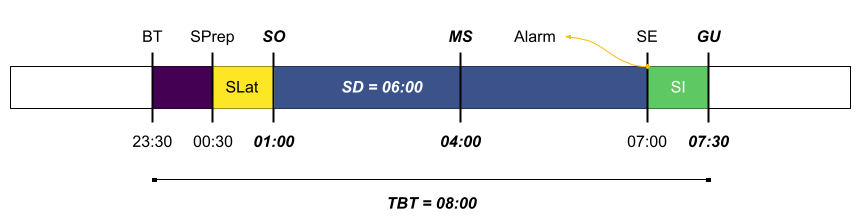
\includegraphics[keepaspectratio]{qmd/images/mctq-figure-1.png}}

\legend{Source: Created by the author.}

}

\end{figure}%

Participants completed an online questionnaire, which included the sleep
log as well as sociodemographic (e.g., age, sex), geographic (e.g., full
residential address), anthropometric (e.g., weight, height), and data on
work and study routines. A version of the questionnaire, stored
independently by the \href{https://archive.org/}{Internet Archive}
organization, can be viewed at
\url{https://web.archive.org/web/20171018043514/each.usp.br/gipso/mctq}.

\subsection{Geographic Parameters}\label{geographic-parameters}

We obtained latitude and longitude data by geocoding participants'
residential addresses using two main resources:

\begin{itemize}
\tightlist
\item
  \href{https://www.qualocep.com/}{QualoCEP} \autocite{qualocep2024}: A
  dataset of Brazilian postal codes with integrated geocoding via the
  Google Geocoding API. This served as our primary source.
\item
  \href{https://developers.google.com/maps/documentation/geocoding/overview}{Google
  Geocoding API}: Used for addresses not included in QualoCEP. We
  employed the
  \href{https://jessecambon.github.io/tidygeocoder/}{tidygeocoder} R
  package \autocite{cambon2021} to facilitate this process.
\end{itemize}

To ensure consistency, we randomly compared results from QualoCEP and
Google Geocoding API. This can be seen in the supplementary materials.

\subsection{Solar Irradiance Data}\label{solar-irradiance-data}

The solar irradiance data came from the
\href{https://labren.ccst.inpe.br/atlas_2017.html}{2017 Solar Energy
Atlas} of Brazil's National Institute for Space Research (INPE)
\autocite{pereira2017}. We used the Global Horizontal Irradiance (GHI)
data, representing the total amount of irradiance received from above by
a surface horizontal to the ground.

\subsection{Astronomical Calculations}\label{astronomical-calculations}

The \href{https://doi.org/10.32614/CRAN.package.suntools}{suntools} R
package \autocite{bivand} was employed to calculate sunrise, sunset
times, and daylight duration for each participant's location. These
calculations are based on equations provided by \textcite{meeus1991} and
the National Oceanic and Atmospheric Administration
(\href{https://gml.noaa.gov/grad/solcalc/calcdetails.html}{NOAA}).

The dates and times of equinoxes and solstices were acquired from the
\href{https://www.timeanddate.com/calendar/seasons.html?year=2000&n=1440}{Time
and Date AS} service \autocite{timeanddateas}. To verify accuracy, we
compared this data with the equations from \textcite{meeus1991} and the
results from the National Aeronautics and Space Administration (NASA)
\href{https://data.giss.nasa.gov/modelE/ar5plots/srvernal.html}{ModelE
AR5 Simulations} \autocite{nasa}.

\subsection{Sample Characteristics}\label{sample-characteristics}

The analysis dataset consisted of \(65,824\) participants aged 18 or
older residing in the UTC-3 timezone. These individuals completed the
survey during a one-week period from October 15th to 21st, 2017,
providing a snapshot of the population at that specific time.

The unfiltered valid sample included \(115,166\) participants from all
Brazilian states. The raw dataset contained \(120,265\) individuals,
with \(98.173\%\) of the responses collected between October 15th and
21st, 2017. This data collection period coincided with the promotion of
the online questionnaire via a
\href{https://globoplay.globo.com/v/6219513/}{broadcast} on a nationally
televised Sunday show in Brazil \autocite{redeglobo2017}.

Based on 2017 data from the Brazilian Institute of Geography and
Statistics's (IBGE) Continuous National Household Sample Survey
(\href{https://www.ibge.gov.br/estatisticas/sociais/trabalho/17270-pnad-continua.html}{PNAD
Contínua}) \autocite{ibgee}, Brazil had \(51.919\%\) of females and
\(48.081\%\) of males with an age equal to or greater than 18 years old.
The sample is skewed for female subjects, with \(66.433\%\) of females
and \(33.567\%\) of male subjects. The mean age was \(32.109\)
(\(\text{SD} = 9.258\)), ranging from \(18\) to \(58.95\) years.

To balance the sample, weights were incorporated into the models. These
weights were calculated through cell weighting, using sex, age group,
and state of residence as references, based on population estimates from
IBGE for the same year as the sample.

A survey conducted in 2019 by IBGE \autocite*{ibge2021} found that
\(82.17\%\) of Brazilian households had access to an internet
connection. Therefore, this sample is likely to have a good
representation of Brazil's population.

The sample latitudinal range is \(33.85026°\)
(\(\text{Min.} = -33.52156°\), \(\text{Max.} = 0.32869°\)) with a
longitudinal span of \(22.74063°\) (\(\text{Min.} = -57.5531°\),
\(\text{Max.} = -34.81247°\)). For comparison, Brazil has a latitudinal
range of \(39.02299°\) (\(\text{Min.} = -33.75115°\);
\(\text{Max.} = 5.27184°\)) and a longitudinal span of \(45.15451°\)
(\(\text{Min.} = -73.99045°\); \(\text{Max.} = -28.83594°\)), according
to data from IBGE collected via the
\href{https://ipeagit.github.io/geobr/index.html\%3E}{geobr} R package
\autocite{pereira}.

Additional details about the sample are available in the supplementary
materials.

\subsection{Power Analysis}\label{power-analysis}

To assess the adequacy of the sample size for detecting effects reaching
the Minimum Effect Size (MES) threshold (\(f^2 = 0.02\)), we conducted
an \emph{a posteriori} power analysis using the
\href{https://cran.r-project.org/web/packages/pwrss/vignettes/examples.html}{pwrss}
R package \autocite{bulus}. This analysis revealed a minimum sample size
of \(1,895\) observations per variable to achieve a power
(\(1 - \beta\)) of \(0.99\) with a significance level (\(\alpha\)) of
\(0.01\). Our sample size (\(n = 65,824\)) comfortably surpasses this
threshold, ensuring adequate power.

\subsection{Data Munging}\label{data-munging}

Data munging and analysis followed the data science framework proposed
by Hadley Wickham and Garrett Grolemund \autocite{wickham2023e}. All
processes were conducted using the R programming language
\autocite{rcoreteama} and several R packages. The
\href{https://www.tidyverse.org/}{tidyverse} and
\href{https://ropensci.org/}{rOpenSci} peer-reviewed package ecosystem
and other R packages adherents of the tidy tools manifesto
\autocite{wickham2023c} were prioritized.

The MCTQ data was analyzed using the
\href{https://docs.ropensci.org/mctq/}{mctq} R package
\autocite{vartanianh}, which is part of the rOpenSci peer-reviewed
ecosystem. The data pipeline was built using the rOpenSci peer-reviewed
\href{https://books.ropensci.org/targets/}{targets} R package
\autocite{landau2021a}, which provides a reproducible and efficient
workflow for data analysis.

All processes were designed to ensure result reproducibility and
adherence to the FAIR principles (Findability, Accessibility,
Interoperability, and Reusability) \autocite{wilkinson2016}. All
analyses are fully reproducible and were conducted using
\href{https://quarto.org/}{Quarto} computational notebooks. The
\href{https://rstudio.github.io/renv/}{renv} R package \autocite{usheya}
was employed to ensure that the R analysis environment can be reliably
restored.

\subsection{Hypothesis Test}\label{hypothesis-test}

To test the study hypothesis, nested multiple linear regression models
were compared: a restricted model (excluding latitude) and a full model
(including latitude). The restricted model included sex, age, longitude,
and the average monthly Global Horizontal Irradiance (GHI) at the time
of questionnaire completion related to the latitude/longitude of each
respondent as predictors. Two full models were tested. The first one
including the restricted predictors plus the average annual GHI (proxy
for the latitude) and daylight duration for the nearest March equinox,
as well as the June and December solstices---all related to the
latitude/longitude of each respondent.The second one included the
restricted model predictors with only the latitude decimal degrees as a
predictor.

It is important to notice that the design of the models were based on
\textcite{leocadio-miguel2017} study. Cell weights were applied to
account for sample imbalances. The models were compared using an F-test
for nested models, with a Type I error probability (\(\alpha\)) of
\(0.05\).

To ensure practical significance, a Minimum Effect Size (MES) criterion
was applied, in line with the original Neyman-Pearson framework for data
testing \autocite{neyman1928,neyman1928a,perezgonzalez2015}. The MES was
set at a Cohen's threshold for small effects (\(f^2 = 0.02\), equivalent
to \(\text{R}^2 = 0.01960784\)) (``just barely escaping triviality''
\autocite[413]{cohen1988a}). Consequently, latitude was considered
meaningful only if its inclusion explained at least \(1.960784\%\) of
the variance in the dependent variable.

The hypothesis can be outlined as follows:

\begin{itemize}
\item
  \textbf{Null hypothesis} (\(\text{H}_{0}\)): Adding \emph{latitude}
  does not meaningfully improve the model's fit, indicated by a
  negligible change in adjusted \(\text{R}^{2}\).
\item
  \textbf{Alternative Hypothesis} (\(\text{H}_{a}\)): Adding
  \emph{latitude} meaningfully improves the model's fit, indicated by an
  increase in adjusted \(\text{R}^{2}\) exceeding the MES.
\end{itemize}

Formally:

\[
\begin{cases}
\text{H}_{0}: \Delta \ \text{Adjusted} \ \text{R}^{2} < \text{MES} \\
\text{H}_{a}: \Delta \ \text{Adjusted} \ \text{R}^{2} \geq \text{MES}
\end{cases}
\]

\medskip

Where:

\[
\Delta \ \text{Adjusted} \ \text{R}^{2} = \text{Adjusted} \ \text{R}^{2}_{\text{full}} - \text{Adjusted} \ \text{R}^{2}_{\text{restricted}}
\]

\medskip

\section{Data Availability}\label{data-availability}

Some restrictions apply to the availability of the main research data,
which contain personal and sensitive information. As a result, this data
cannot be publicly shared. Data are, however, available from the author
upon reasonable request.

The code repository is available on GitHub at
\url{https://github.com/danielvartan/mastersthesis}, and the research
compendium can be accessed via \href{https://osf.io/}{The Open Science
Framework} at the following link:
\url{https://doi.org/10.17605/OSF.IO/YGKTS}.

\section{Acknowledgments}\label{acknowledgments}

This study was financed in part by the Coordenação de Aperfeiçoamento de
Pessoal de Nível Superior - Brasil
(\href{https://www.gov.br/capes/}{CAPES}) - Finance Code 001, Grant
number 88887.703720/2022-00.

\section{Ethics Declaration}\label{ethics-declaration}

The author declares that the study was carried out without any
commercial or financial connections that could be seen as a possible
competing interest.

\section{Additional Information}\label{additional-information}

See the supplementary material for more information.

Correspondence can be sent to Daniel Vartanian
(\href{mailto:danvartan@gmail.com}{\nolinkurl{danvartan@gmail.com}}).

\section{Rights and Permissions}\label{rights-and-permissions}

This article is released under the
\href{http://creativecommons.org/licenses/by/4.0/}{Creative Commons
Attribution 4.0 International License}, which permits use, sharing,
adaptation, distribution, and reproduction in any medium or format, as
long as be given appropriate credit to the original author and the
source, provide a link to the Creative Commons license, and indicate if
changes were made.

\bookmarksetup{startatroot}

\chapter{Conclusion}\label{sec-conclusion}

\epigraph{Every genuine test of a theory is an attempt to falsify it, or to refute it.}{--- \textcite{popper2002}}
\vspace*{-1\baselineskip}
\epigraph{I suggest that it is the aim of science to find satisfactory explanations, of whatever strikes us as being in need of explanation.}{--- \textcite[193]{popper1979a}}
% \vspace*{1\baselineskip}

The preceding chapters have presented a comprehensive examination of
evidence and analyses pertaining to the latitude hypothesis in
chronobiology. At this juncture, it is essential to return to the
fundamental research question that motivated this thesis: \emph{Is
latitude associated with chronotype?}

This study, using what is arguably one of the largest datasets on
chronotype, found no evidence supporting the latitude hypothesis in
humans.

Current evidence does not support the latitude hypothesis, and some
claims made in its favor warrant further examination (see Supplemental
Materials). Nevertheless, the hypothesis is often cited in chronobiology
research as if it were well-established. While this study does not
definitively refute it, the relationship between latitude and chronotype
should remain an open scientific question until strong evidence
substantiates it.

\section{Strengths}\label{strengths}

Testing any theory or hypothesis is inherently challenging and often
sparks debate. In this context, it is important to acknowledge the
significant strengths of this study:

\begin{itemize}
\tightlist
\item
  \textbf{Large, focused sample}: One of the largest chronotype datasets
  ever collected within a single time zone (\(n = 65,824\)).
\item
  \textbf{Minimal photoperiod variability}: Data were collected over a
  single spring week as summer approached (October 15--21, 2017),
  effectively controlling for seasonal variations in daylight exposure
  across regions.
\item
  \textbf{Broad latitudinal range}: The sample spans a considerable
  range (\(33.85°\)).
\item
  \textbf{Population balancing}: The dataset was adjusted to reflect
  population proportions at the time of collection.
\item
  \textbf{Rigorous statistical analysis}: The study accounted for
  confounders and incorporated a practical significance threshold.
\item
  \textbf{Full reproducibility}: All analyses, from raw data processing
  through effect size estimation, follow transparent and reproducible
  protocols available for verification.
\end{itemize}

It is also worth noting that, despite methodological improvements, this
study is grounded in the same core principles and variables that
underpin the latitude hypothesis. Consequently, any critique of its
methods should be considered in light of the methods used by studies
that support the hypothesis.

\section{Limitations}\label{limitations}

While this study provides valuable evidence, certain limitations should
be acknowledged, as they may influence the interpretation of the
findings:

\begin{itemize}
\tightlist
\item
  \textbf{Self-report biases}: The Munich Chronotype Questionnaire
  (MCTQ), despite being a validated instrument, is subject to recall and
  social desirability biases inherent in self-reported measures. The
  large sample size likely mitigates these biases, as suggested by the
  law of large numbers \autocite[352]{degroot2012a}.
\item
  \textbf{Validation in portuguese}: At the time of data collection, the
  MCTQ had not been officially validated in Portuguese (a process
  completed in 2020 by \textcite{reis2020a}), potentially introducing
  minor inconsistencies. However, given its sleep log format, the impact
  is expected to be minimal.
\item
  \textbf{Daylight Saving Time (DST)}: The timing of data collection
  coincided with the onset of Daylight Saving Time (DST) in Brazil. On
  October 15th, 2017, the day data collection commenced (\(80.153\%\) of
  the data used in this analysis were collected on this day), a
  significant portion of respondents adjusted their clocks forward by
  one hour. Although this adjustment could theoretically influence
  responses, the questions were designed to capture daily routines that
  were not directly affected by the DST shift. Furthermore, if DST had
  any effect, it would have been expected to bolster the latitude
  hypothesis; yet, this was not supported by the data.
\item
  \textbf{Latitudinal range}: The latitudinal range of \(33.85°\), while
  substantial, could be questioned as potentially insufficient to detect
  latitude effects on chronotype. However, the absence of a meaningful
  association within this range suggests that any such effect, if
  present, would be minimal.
\item
  \textbf{Unexamined confounders}: Although key confounders were
  controlled for, some variables remained unexamined (e.g.,
  socioeconomic status, urbanization, social timing). While including
  these variables might enhance model precision, it could also introduce
  multicollinearity and overfitting concerns. In the context of the
  tested hypothesis, the exclusion of these additional predictors is
  unlikely to alter the overall conclusions.
\item
  \textbf{Chronotype measurement}: The study used sleep as a proxy for
  measuring chronotype, leveraging its underlying circadian processes.
  However, sleep is not the only marker of circadian phenotypes. More
  precise methods, such as Dim Light Melatonin Onset (DLMO)
  \autocite{ruiz2020}, can provide a direct measure of circadian phase.
  Yet, these approaches are often more invasive and costly, limiting
  both sample size and the generalizability of findings.
\item
  \textbf{Generalizability}: Finally, the study's generalizability is
  limited to the Brazilian population. However, since the latitude
  hypothesis's underlying principles are not geographically constrained,
  these findings provide valuable insights for future research in other
  regions.
\end{itemize}

These limitations, while important to consider, do not undermine the
study's findings; rather, they highlight areas where future research
might further refine our understanding.

\section{Directions for Future
Research}\label{directions-for-future-research}

This thesis proposed using a global modeling approach to investigate the
latitude-chronotype relationship. As demonstrated by the results of this
study and others, no meaningful effect of latitude on chronotype was
identified. That said, it remains possible that if such a phenomenon
exists, it could be captured through a localized approach, such as
agent-based modeling. This approach would simulate an environment where
agents are exposed to varying light levels, while accounting for their
endogenous rhythms and the circadian clock's phase-response curve to
light. The data from this thesis could serve to calibrate and validate
this model.

\postextual

\begingroup
\renewcommand{\baselinestretch}{1}
\setcounter{footnote}{0}
\renewcommand{\thefootnote}{\fnsymbol{footnote}}
\printbibliography[heading=bibheading]
\endgroup

\tocskipone
\tocprintchapternonum
\addcontentsline{toc}{chapter}{\newbibname}

% -----
% Other additions
% -----

%:::% other-after-body begin %:::%
%:::% other-after-body end %:::%

\end{document}
